%\section{Cohesive sediment}\label{ch:cohesive}%\footnote{This chapter has been written by D. Phan van Bang, Lan and Villaret}

\section{Introduction}

Fine cohesive sediments are predominant in most estuaries, basins and reservoirs.
The prediction of cohesive sediment transport, often associated with pollutants, is crucial
regarding environmental issues. 

Complex properties - floculation and consolidation - strongly affect the dynamic behavior of cohesive particles. 
We describe in this chapter the cohesive sediment treatment in \sisyphe.
This chapter is organized as follows:
we start in Section ? with a general presentation of cohesive sediment properties and floculation processes.
As a result of consolidation, cohesive beds are generally stratified. This effect is represented by a multi-layer model described in section . The next section presents the 2D suspended sediment tranpsort equation. 
The bed evolution is obtained to balance the net erosion-deposition flux, as described in the next Section?.
The last Section ? is devoted to the consolidation algorithms.
Appendix 1 gives a list of keywords for cohesive applications and user-subroutines. In
Appendix 2, the Gibson equation is derived for consolidation modelling


\section{Cohesive properties}

\subsection{Cohesive/non-cohesive sediment}


For non-cohesive sediments (sand and gravel), the grain size distribution and particle properties (
 density $\rho_s$ and shape) determine its
resistance to erosion, settling velocity and transport rate. Non-
cohesive material are generally made of quartz, such that the density of
sand particles is approximately constant and around 2650 kg/m$^{3}$. 
Non-cohesive sand particles can be transported as bed-load or suspended load. 
They can be represented by a finite number of
classes, each characterized by its mean diameter, grain density and constant
settling velocity (see previous Chapter). 


Cohesive properties 
appear for fine particles (silts and clay), with diameter less than a limiting value of about 60 $\mu$m, depending on the physico-chemical 
properties of the fluid and salinity.
Fine cohesive sediments are transported in suspension (no bed-load).
Transport processes 
strongly depend on the state of floculation of the suspension and consolidation of the bed.
the erosion rate mainly depends on the degree of consolidation of the sediment bed, 
while the settling velocity depends on the state of floculation and aggregates properties.


\begin{bclogo}[couleur = blue!10, arrondi = 0.10, logo = \bcattention]{\textsf{Attention}}
The separation value at $60\mu$m to discriminate non-cohesive from
cohesive sediment is conventional (UK classification). The value is
different depending on the country ($63\mu$m in Netherlands, $75\mu$m in USA
as pointed by Winterwerp and Van Kesteren, 2004). Moreover, aggregation of
flocs can lead to the formation of macro-flocs larger than $100\mu$m.
\end{bclogo}



\medskip
\begin{bclogo}[couleur=blue!10,arrondi=0.1, logo=\bcinfo]{Keywords}
We consider in Sisyphe, the simpler case of uniform, cohesive sediments,
characterized by one single value for the primary grain size $D_{50}$ and
density $\rho_s=2650$ kg/m$^{3}$ for quartz particles, which is
transported in suspension (no bedload).

In the \sisyphe steering file, the physical properties of the sediment are
defined:
\begin{itemize}
\item {\ttfamily COHESIVE SEDIMENT = YES} ({\ttfamily = NO}, default option)
\item {\ttfamily SEDIMENT DIAMETERS} ($D_{50} > 0.00006$ m, for non-cohesive sediment)
\item {\ttfamily SEDIMENT DENSITY} ($\rho_s = 2650$ Kg/m$^3$, default value)
\end{itemize}

Both key words \texttt{SUSPENDED LOAD = YES}, \texttt{BED LOAD = NO} are
set automatically, in order to be consistent with the selected type of
sediment, when \texttt{COHESIVE SEDIMENT = YES}

\begin{itemize}
\item {\ttfamily SUSPENDED LOAD = YES} ({\ttfamily = NO}, default option)
\item {\ttfamily BED LOAD = NO} ({\ttfamily = YES}, default option)
\end{itemize}
\end{bclogo}



\subsection{Effect of floculation}


For cohesive sediments ($D_{50} < 60 \mu$m), the primary grain
diameter and density no longer control the transport rates. Due to electro-static
attractive forces (van der Waals), individual particles tend to form flocs.
Their size can be an order of magnitude greater than the initial particle
diameter, while the density decreases: the floc characterictics (size and
density, as well as its fractal dimension) are more relevant to compute the settling velocity (cf. Van Leussen, ???).

The settling velocity of cohesive particles therefore depends on the
suspended sediment concentration as well as on other physico-chemical
properties (pH, salinity, cations for instance) of the suspension which
influence the flocculation process. The effect of turbulence level
determines also the floculation state. The critical bed shear strength
depends on the consolidation state or age of the sediment bed (Migniot,
1968).

Floculation can be modelled using process based models (cf. Mc Anally, 1999, Klassen et al. 2013).
The settling velocity is generally an
order of magnitude greater than the settling velocity based on the individual
particle size, as a result of flocculation.

The flocculation process is not yet programmed in \sisyphe and the settling
velocity should be specified by the user as a calibration parameter. 
More physically based relations will be
implemented in the future. 


\begin{bclogo}[couleur = blue!10, arrondi = 0.10, logo = \bcattention]{\textsf{Attention}}
 The settling velocity needs to be specified, if not, it will
be calculated by the Stokes law as a function of the individual particle
diameter in subroutine \texttt{vitchu\_sisyphe.f}. As a result of flocculation, the
settling velocity can be approximately an order of magnitude greater. 
\begin{itemize}
\item {\ttfamily SETTLING VELOCITIES}
\end{itemize}
\end{bclogo}



\subsection{Consolidation process}\label{sec:4.1}

Once the sedimentation process is achieved, a sediment bed is formed. For
non-cohesive bed, no evolution with time will be observed if no erosion or
further sedimentation occurs. For cohesive bed, the concentration will
increase with time as the result of self-weight consolidation or compaction.
Two stages, namely the primary and secondary consolidation (Been and Sills,
1981), are classically considered to explain the progressive compaction of
the cohesive sediment bed with time. As the formed bed resulting from the
sedimentation of mud is very soft, it tends to compact under its
self-weight. During this process, the void ratio tends to diminish so that
pore water is expulsed upward as a result of water incompressibility. The
dynamic of this primary stage of consolidation is therefore controlled by
the permeability of the bed. At the end of the primary consolidation, the
excess pore pressure is fully dissipated (Figure~\ref{fig:2}) but the cohesive bed
records further compaction. This secondary stage of consolidation is no
longer related to pore pressure but rather to the solid skeleton property.
The secondary consolidation is considered as a result of time effect
(viscous or ageing) in the stress-strain relationship of the soil. Two
effects of time are currently considered in modern soil mechanic: the creep
of the soil (viscous behaviour of cohesive geomaterial) and ageing
(thixotropy of mud). Even through the dynamic of the secondary consolidation
is much slower than the primary consolidation, this stage is important for
long term prediction.

\pagebreak

\begin{figure}[htb]
\begin{center}
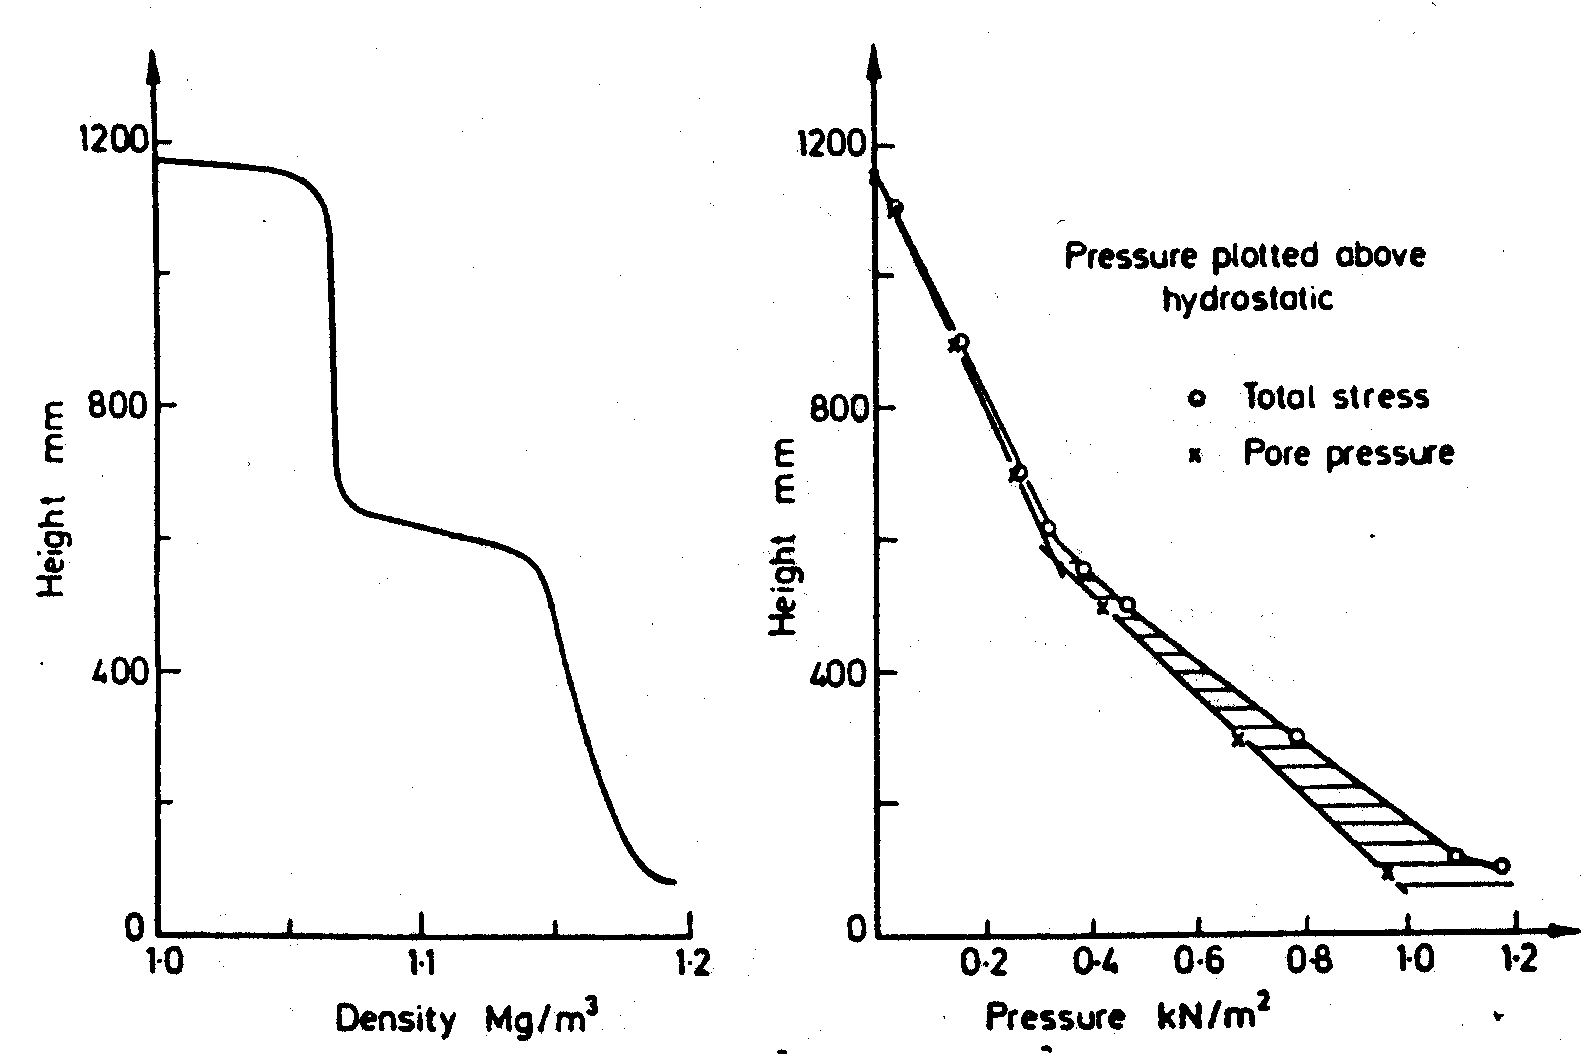
\includegraphics[scale=1.0,angle=0]{graphics/fig2.png}
\caption{Vertical variation of density and effective stress within the
cohesive sediment bed.}\label{fig:2}
\end{center}
\end{figure}


\subsection{Multi-layer model}


Cohesive sediment beds are generally non-uniform: as a result of
self-weight consolidation, the bed becomes stratified, with density
increasing with distance from the surface. The top layer is generally made
of freshly deposited soft mud, while the bottom consolidated layers present
higher resistance to erosion. The vertical
stratification of the cohesive bed is therefore a key issue, which controls the
amount of material to be put in suspension. 

In \sisyphe, cohesive sediment bed can be represented by a fixed number
\texttt{NCOUCH\_TASS} of layers. The number of
layers is fixed with maximum number up to $20$. Each layer is characterized by its 
concentration and resitance to erosion. The concentration of each layer ($C_s (j)$)is generally constant
and specified by keyword \texttt{MUD CONCENTRATION PER LAYER} expressed in kg/m$^3$. It
may also vary in space and time (see consolidation model 3).
The resistance of each layer is specified by keyword \texttt{CRITICAL EROSION SHEAR STRESS OF THE MUD} expressed in N/m$^2$.

\begin{figure}[ht]
\label{fig:1}
\begin{center}
\begin{tabular}{c}
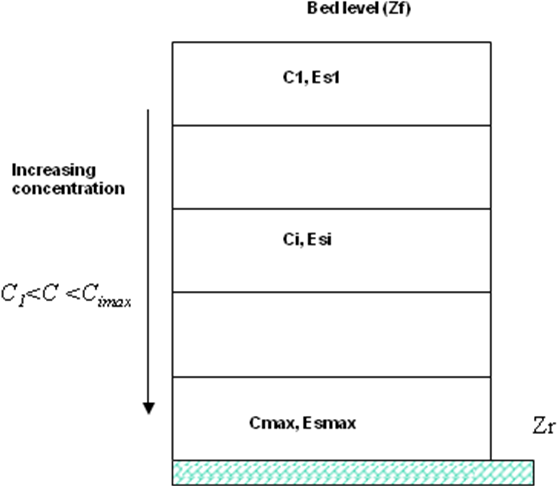
\includegraphics[scale=1.0]{graphics/vertical_bed_structure.png} %&
\end{tabular}
\caption{Multi-layer bed structure (\texttt{NCOUCH\_TASS} is the number of layers)}
\end{center}
\end{figure}


Each layer $j$ ($1 \leq j \leq NCOUCH\_TASS$) is defined by its concentration $C_s$, thickness $E_s$ and mass per surface area $M_s$, 
which depends on both layer concentration and thickness, such that
\begin{equation*}
M_s(i,j) = C_s(j) E_s(i,j)
\end{equation*}
where $M_s$ is the mass per unit surface area (Kg/m$^2$), $C_s$ is the concentration (kg/m$^3$) and $E_s$ the layer thickness.

For particular application, the bed concentrations $C_s(i, j)$ can be
also allowed to vary from point to point. The initial distribution can be
specified in subroutine \texttt{init\_compo\_coh.f}. 

\medskip
\begin{bclogo}[couleur=blue!10,arrondi=0.1, logo=\bcinfo]{Keywords}
\begin{itemize}
\item {\ttfamily NUMBER OF LAYERS OF THE CONSOLIDATION MODEL} : $NCOUCH\_TASS$ (default value $= 1$)  should be less than the maximum number of layers ({\ttfamily NLAYMAX = 20})
\item {\ttfamily MUD CONCENTRATION PER LAYER}, in Kg/m$^3$: $ CONC\_VASE$
\end{itemize}
\end{bclogo}

\begin{bclogo}[couleur = blue!10, arrondi = 0.10, logo = \bcattention]{\textsf{Attention}}
The keywords {\ttfamily NUMBER OF BED LOAD MODEL LAYERS} and
{\ttfamily NUMBER OF LAYERS OF THE CONSOLIDATION MODEL} are essentially the same
except that the default values are different. 

For cohesive sediments, it is possible to have only one uniform layer, whereas for sand grading algorithm
we need at least 2 layers (the active layer and the substratum).
The subroutine {\ttfamily lecdon.f} specifies at the end $NOMBLAY = NCOUCH\_TASS$
\end{bclogo}
\begin{bclogo}[couleur = blue!10, arrondi = 0.10, logo = \bcattention]{\textsf{Attention}}
Due to the default value of $NOMBLAY$ for sand grading
effects ($NOMBLAY = 2$).
For uniform beds both keywords need to be specified:
\begin{itemize}
\item {\ttfamily NUMBER OF BED LOAD MODEL LAYERS = 1}
\item {\ttfamily NUMBER OF LAYERS OF THE CONSOLIDATION MODEL = 1}
\end{itemize}
\end{bclogo}



\pagebreak
\section{Suspended load}

%subsection{Erosion and deposition laws}

%Cohesive sediments are transported only in suspension (no bedload), such
%that the Exner equation for the bed evolution is no-longer solved. The bed
%evolution is obtained as a mass balance between the erosion and deposition
%fluxes, which can be calculated  using the Krone and Partheniades erosion/deposition
%laws: erosion fluxes need a specific treatment in order to correctly account
%for the increase of bed shear strength as the bed gets eroded down
%to the deeper consolidated layers.


\subsection{2D Transport equation}
Fine cohesive sediments are transported in suspension (no bedload), such
that the Exner equation for the bed evolution is no-longer solved. The two-dimensional
(2D) model solves a two-dimensional (2D) transport equation for the
depth-averaged suspended sediment transport concentration $C$, which is
derived by depth-integration of the 3D classical transport/diffusion
equation.

\begin{equation*}
X=\overline{x} = \frac{1}{h} \int_{Z_f}^{Z_s} x(z) d z 
\end{equation*}
where $h = Z_s - Z_f$ is the water depth, assuming the bed-load layer
thickness to be small.

After simplification of the advection terms and using the continuity
equation, the following approximate depth-averaged transport equation can be
solved in its non-conservative form:

\begin{equation*}
\frac{\partial C}{\partial t} + 
\underbrace{U\frac{\partial C}{\partial x} + V\frac{\partial C}{\partial y}}_{\text{advection}} = 
\underbrace{\frac{1}{h}\left[\frac{\partial}{\partial x}\left(h\epsilon_s\frac{\partial C}{\partial x}\right) + 
\frac{\partial}{\partial y}\left(h\epsilon_s\frac{\partial C}{\partial y}\right) \right]}_{\text{diffusion}} + 
\frac{(E-D)}{h}
\end{equation*}
where $U$ and $V$ are the depth-averaged convective flow
velocities in the $x$ and $y$ directions, $E$ and $D$ are respectively the erosion and
deposition fluxes at the bed and represent the exchange terms between the
suspension and the sediment bed. They are defined at the interface between
the bed and the suspension.

\begin{bclogo}[couleur = blue!10, arrondi = 0.10, logo = \bcattention]{\textsf{Attention}}
In \sisyphe, the volume concentration is the main variable such that $E$ and $D$
are expressed in m/s. However, the user can choose mass concentration for graphic printouts, by
use of keyword \texttt{MASS CONCENTRATION}.
The relation between volume concentration $C$ and mass concentration $C_s$
(Kg/m$^3$) is $C_s = \rho_s C$, where $\rho_s$ is the solid
density ($\rho_s = 2650$ Kg/m$^3$)
\end{bclogo}

\subsection{Convection/Diffusion terms}
\subsubsection{Convection}
For non-cohesive sediments, the convective velocity generally differs from
the depth-averaged velocity (issued from \teldd). A correction term is
applied on the depth-averaged mean velocity to account for the fact that
most sediments is transported near the bed. This correction term is
expressed as a function of the Rouse parameter as explained in the
user-manual (cf. Report H-P74-2012-02004-EN). 

For fine cohesive sediments, the Rouse parameter:
\begin{equation*}
R=\frac{w_s}{\kappa u_*} 
\end{equation*}%
where $w_s$ is the settling velocity, $\kappa$ the von Karman constant ($\kappa=0.4$), and $u_*$ 
the friction velocity is generally less than
one and the sediment can be regarded as fairly uniformly distributed in the
vertical. The convection velocity can be taken as the depth-averaged flow
velocity.

\subsubsection{Diffusion}
The horizontal diffusion terms can be set to zero by use of keyword
\texttt{DIFFUSION = NO}. The expression of the diffusion term depends on the choice of parameter \texttt{OPDTRA} (keyword).
For \texttt{OPDTRA=1}, the diffusion
terms in (2) can be simplified as follows:

\begin{equation}
\frac{\partial C}{\partial t} + 
U \frac{\partial C}{\partial x} + 
V\frac{\partial C}{\partial y} = 
\left[\frac{\partial}{\partial x} \left(\epsilon_s\frac{\partial C}{\partial x}\right) + 
\frac{\partial}{\partial y}
\left(\epsilon_s \frac{\partial C}{\partial y} \right)\right] + 
\frac{(E-D)}{h} 
\end{equation}

\medskip
\begin{bclogo}[couleur=blue!10,arrondi=0.1, logo=\bcinfo]{Keywords}
In the \sisyphe steering file, the physical properties of the sediment are
defined:
\begin{itemize}
\item {\ttfamily CORRECTION ON CONVECTION VELOCITY} ({\ttfamily = NO}, default option)
\item {\ttfamily MASS CONCENTRATION} ({\ttfamily = NO}, default option)
\item {\ttfamily OPTION FOR THE DIFFUSION OF TRACER} ({\ttfamily OPDTRA = 1}, default option)
\end{itemize}
\end{bclogo}

\subsubsection{Numerical schemes}

The choice of the numerical scheme is based on keyword \texttt{TYPE OF
ADVECTION}. The following numerical methods are available in \sisyphe:
\begin{itemize}
\item \textbf{Method of characteristics} (\texttt{1}) 
\begin{itemize}
\item Unconditionally stable and monotonous
\item Diffusive for small time steps
\item Not mass conservative
\end{itemize}
\item \textbf{Method Streamline Upwind Petrov Galerkin SUPG} (\texttt{2}) 
\begin{itemize}
\item Courant number criteria
\item Not mass conservative
\item Less diffusive for small time steps
\end{itemize}
\item \textbf{Conservative N-scheme (similar to finite volumes)} (\texttt{3, 4})
\begin{itemize}
\item Solves the continuity equation under its conservative form
\item Recommended when the correction on convection velocity is

accounted for
\item Courant number limitation (sub-iterations are included to
reduce the time step
\end{itemize}
\item Numerical schemes \texttt{13} and \texttt{14} are the same as \texttt{3} and \texttt{4} 
but here adapted to the presence of tidal flats based on positive water depth algorithm 
\item \textbf{Distributive schemes (PSI)} 
\begin{itemize}
\item like scheme 4, but the fluxes are corrected according to the tracer value: this
relaxes the courant number criteria and it is also less diffusive than
scheme \texttt{4} and \texttt{14}
\item The CPU time is however increased 
\item This method should not applied for tidal flats
\end{itemize}
\end{itemize}

\medskip
\begin{bclogo}[couleur = blue!10, arrondi = 0.10, logo = \bcattention]{\textsf{Attention}}
It is recommended to use scheme \texttt{4} or \texttt{14} (if tidal flats are present) as a good
compromise (accuracy/computational time)

\end{bclogo}

\medskip
\begin{bclogo}[couleur=blue!10,arrondi=0.1, logo=\bcinfo]{Keywords}
\begin{itemize}
\item {\ttfamily TETA SUSPENSION} ({\ttfamily = 1}, default option)
\item {\ttfamily TYPE OF ADVECTION} ({\ttfamily = 1}, default option)
\item {\ttfamily SOLVER FOR SUSPENSION} ({\ttfamily = 3}, conjugate gradient by default option)
\item {\ttfamily PRECONDITIONING FOR SUSPENSION} ({\ttfamily = NO}, default option)
\item {\ttfamily SOLVER ACCURACY FOR SUSPENSION} ($1.0\times 10^{-8}$, default option)
\item {\ttfamily MAXIMUM NUMBER OF ITERATIONS FOR SOLVER FOR
SUSPENSION} ({\ttfamily = 50}, default option)
\item {\ttfamily OPTION FOR THE DISPERSION} ({\ttfamily = 1}, constant
dispersion coefficient by default option)
\item {\ttfamily DISPERSION ALONG THE FLOW} ($1.0\times 10^{-2}$, default option)
\item {\ttfamily DISPERSION ACROSS THE FLOW} ($1.0\times 10^{-2}$, default option)
\end{itemize}
\end{bclogo}


\section{Bed evolution}

\subsection{Mass balance equation}



The bed evolution
is only due to the suspended load (no bed-load). The following mass balance equation is 
solved at each time step:
\begin{equation}
C_s \frac{\partial Z_f}{\partial t} + \rho_s (E-D) = 0 
\end{equation}%
where $Z_f$ is the bottom elevation (m), $C_s$ is the mass concentration of the cohesive
bed which increases from the top layer to the bottom in the multi-layer
discretization of the bed (Kg/m$^3$), $E-D$ is the net erosion minus deposition flux (m/s) and 
$\rho_s$ is the solid particles density (kg/m$^3$).

The subroutine \texttt{evol\_susp\_coh.f} updates the bed level $dZ_f$ and layer
thicknesses $E_s$, as well as the mass of mud per layer $M_s$. 

\subsection{Erosion Flux}
 Erosion fluxes can be calculated using the the Parthenides classical formula which is programmed in \sisyphe: erosion flux can 
be related to the excess of applied bed shear stress to the bed shear strength at the bed surface. 
When the bed is stratified, it is necessary to take into account
the vertical increase of bed shear strength as the bed gets eroded.
\subsubsection*{Uniform bed ($NCOUCH\_TASS = 1$)}
The classical Partheniades formula is applied for cohesive sediments.
Assuming the bed to be uniform: 
\begin{equation*}
E = \left\{\begin{array}{ll}
\displaystyle
M\left(\left(\frac{u_*}{u_{*e}}\right)^2-1\right) & \quad \text{if } u_* > u_{*e} \\
\displaystyle
0 & \quad \text{otherwise} 
\end{array}
\right.
\end{equation*}
where $u_{*e}$ is the critical erosion velocity and $u_*$ is the friction velocity related to skin
friction, defined as: 
\begin{equation*}
u_* =\sqrt{\frac{\tau'}{\rho}} 
\end{equation*}%
with $\tau'$ the bed shear stress corrected for skin
friction and $\rho$ the fluid density.

The empirical coefficient $M$ is a dimensional coefficient. The Partheniades
coefficient $M$ is specified in the steering file (in Kg/m$^2$/s). The
erosion rate is expressed in m/s, by converting the $M$ coefficient to m/s
(subroutine \texttt{lecdon.f}).

\subsubsection*{Non uniform bed ($NCOUCH\_TASS > 1$)}
In the multi-layer model, the critical erosion shear stress increases as the
mud concentration increases (see  Migniot, 1968).
%\begin{equation*}
%\tau_{ce} = \rho u_{*e}^2 \approx C^{\beta} 
%\end{equation*}
%where $\tau_{ce}$ is the critical erosion bed shear
%stress, $C$ is the mud concentration, and $\beta$ is an empirical coefficient.

In the multi-layer model, each layer is characterized by its density and
critical bed shear stress. The erosion rate of each layer $E(j)$ decreases with distance from the surface.

For each layer $j$ and at each time step, the erosion rate $E(j)$ is calculated
as a function of the difference between the applied bed shear stress and the
critical bed shear strength, using (4). For each $E(j) > 0$, the layer
is erodible.

The erosion flux $E$ is determined as the mean erosion rate, averaged
over the eroded depth :

\begin{equation*}
E = \frac{1}{\Delta zer} \int_0^{\Delta zer} E(z) dz = \frac{1}{\rho_s dt}
\int_0^{dt} dM_s 
\end{equation*}
where $dM_s$ is the eroded mass per unit surface
area (Kg/m$^2$), $\Delta zer$ is the maximum depth to be eroded, 
$E(z)$ is the erosion flux (m/s) at distance $z$ from
the bed interface, and $dt$ the time step.

\subsubsection*{Iterative procedure}
The potential depth to be eroded is estimated using the iterative procedure
described below and programmed in subroutine \texttt{suspension\_erosion\_coh.f}.

At each time step, the top layer is first eroded if $E(1) > 0$. Once it
is empty, the next layer is eroded etc... For each erodible layer $j$ with
erosion rate ($E(j) > 0$), the time interval $dt(j)$ to erode it
completely is estimated by a simple mass balance from the mass of the layer
$M_s(j)$:
\begin{equation*}
dt(j)=\frac{M_s(j)}{\rho_s E(j)} =\frac{E_s(j) C_s(j)}{\rho_s E(j)} 
\end{equation*}
For the first layer ($j=1$), there are two possibilities: 
\begin{itemize}
\item $dt(1) > dt$: layer $1$ is emptied partially, such that $-C_s(1) dE_s(1)=\rho_s dt E(j)$ 
\item $dt(1) < dt$ : layer $1$ is emptied completly, and the next (second) layer can be eroded, such that $dE_s(1)=-E_s(1)$. 
\end{itemize}
The last (non-empty) layer (noted $j_{max}$) to be eroded is obtained by
emptying all successive top layers until :

\begin{equation*}
\sum_{j=1}^{j_{\max-1}} dt(j) < dt <\sum_{j=1}^{j_{\max}} dt(j) 
\end{equation*}
For $j_{\max}$, the time left to erode the last layer is

\begin{equation*}
dt_{\max} = dt-\sum_{j=1}^{j\max-1} dt(j) 
\end{equation*}%
The mass potentially eroded during this process is

\begin{equation*}
\overline{M_s} = \sum_{j=1}^{j\max-1} M_s(j) + \rho_s E(j_{\max}) dt_{\max} 
\end{equation*}
The erosion flux (m/s) is therefore estimated as follows: 

\begin{equation*}
E=\frac{\overline{M_{s}}}{\rho_s dt} 
\end{equation*}

\medskip
\begin{bclogo}[couleur=blue!10,arrondi=0.1, logo=\bcinfo]{Keywords}
\begin{itemize}
\item {\ttfamily COHESIVE SEDIMENTS} ({\ttfamily = NO}, default option)
\item {\ttfamily PARTHENIADES CONSTANT} ($M = 1\times 10^{-3}$ Kg/m$^2$, default option)
\item {\ttfamily CRITICAL EROSION SHEAR STRESS OF THE MUD} ($\tau_{ce} = 0.01$ N/m$^2$, default option)
\end{itemize}
\end{bclogo}

\subsection{Deposition flux }

The deposition flux is calculated as a function of the near bed
concentration. In the case of fine cohesive sediments ($w_s<< u_*$  where $w_s$ is the settling velocity, and 
$u_*$, the turbulent friction velocity), the bed concentration is approximately equal
to the depth-averaged concentration.  The
deposition flux can be treated as an implicit term in equation (3), whereas the erosion flux is
explicit.

\begin{equation*}
D = \left\{\begin{array}{ll}
\displaystyle
0 & \quad \text{if } u_* > u_{*d} \\
\displaystyle
w_s C\left(1-\left(\frac{u_*}{u_{*d}}\right)^2\right) & \quad \text{otherwise} 
\end{array}
\right.
\end{equation*}
where $C$ is the depth-averaged concentration, $w_s$, the settling velocity, and 
$u_{*d}$, the critical deposition velocity which
represents the limiting shear velocity, above which the sediment flocs are
broken and resuspended.

\medskip
\begin{bclogo}[couleur = blue!10, arrondi = 0.10, logo = \bcattention]{\textsf{Attention}}
In Eq(5), the sediment concentration is assumed to be uniform over depth,
which is a reasonable assumption for fine cohesive sediments ($w_s << u_*$).
\end{bclogo}

\medskip
\begin{bclogo}[couleur=blue!10,arrondi=0.1, logo=\bcinfo]{Keywords}
\begin{itemize}
\item {\ttfamily CRITICAL SHEAR VELOCITY FOR MUD DEPOSITION} ($VITCD = 1000$ m/s, default option)
\item {\ttfamily SETTLING VELOCITIES} (by default, $w_s$ is
calculated by the model based on the Stokes law and individual particle
diameter)
\end{itemize}
\end{bclogo}

\subsection{Bed Evolution}


\subsubsection{Uniform bed ($NCOUCH\_TASS = 1$)}
The bed is characterized by a single density $C_s = C_s(1)$. The bed
evolution at each time step is therefore:

\begin{equation*}
dZ_f =\frac{\rho_s (D-E) dt}{C_s} 
\end{equation*}
($dZ_f < 0$ for net erosion and $dZ_f < 0$ for net
deposition).

\subsubsection{Non-uniform beds ($NCOUCH\_TASS > 1$)}
Two different cases occur. In the case of net deposition ($D-E > 0$),
sediment is deposited in the first top layer $C_s(1)$:

\begin{equation*}
dZ_f = dE_s(1) = \frac{\rho_s(D-E)dt}{C_s(1)} > 0 
\end{equation*}

In the case of net erosion ($E-D > 0$), sediment is eroded layer by
layer $dE_s(j) < 0$, from the surface to the bottom dense layer, until
the eroded mass balances the eroded flux:

\begin{equation*}
\sum_{j=1}^{j\max} M_s(j) = \rho_s(E-D) dt 
\end{equation*}
where $j_{\max}$ is the last layer to be eroded, and $M_s(j)$ is the total mass per surface area of
layer $j$, such that $M_s(j) = C_s(j) E_s(j)$. The last layer to be eroded $j_{\max}$ is determined in order to satisfy:

\begin{equation*}
\sum_{j=1}^{j\max-1} M_s^{n}(j) < \rho_s(E-D)dt < \sum_{j=1}^{j\max} M_s^n(j)
\end{equation*}

Top layers are emptied ($dE_s(j) =-E_s(j)$ for $j=1$ to $j_{\max}-1$); the
last layer is eroded up to a the depth $dE_s(j_{\max}) < 0$ in order to
satisfy mass conservation:

\begin{equation*}
\underbrace{\sum_{j=1}^{j\max-1} M_s^n(j) - dE_s(j_{\max})C_s(j_{\max})}_{\text{eroded mass}} = \rho_s (E-D) dt 
\end{equation*}

The variation of bed elevation is therefore:

\begin{equation*}
dZ_f =-\left(\sum_{j=1}^{j\max-1} E_s^n(j)\right) + dE_s(j_{\max}) < 0 
\end{equation*}
The thickness and mass of each layer are updated at the end of each time
step ($n+1$), from their initial values ($n$):

\begin{equation*}
\text{for}\,j=(1,j_{\max}-1)\,\,\left\{ 
\begin{array}{l}
E_s^{n+1} s(j) = 0 \\ 
M_s^{n+1}(j)=0
\end{array}
\right. 
\end{equation*}
and
\begin{equation*}
for\,j=j_{\max} \left\{ 
\begin{array}{l}
E_s^{n+1} (j_{\max}) = E_s^n(j_{\max}) + dE_s(j_{\max}) \\ 
M_s^{n+1} (j_{\max}) = E_s^{n+1}(j_{\max}) C_s(j_{\max})
\end{array}
\right.
\end{equation*}

Underneath layers (from $j_{\max} + 1$ to $NCOUCH\_TASS$) are not eroded and keep
their thickness and mass.

\medskip
\begin{bclogo}[couleur=blue!10,arrondi=0.1, logo=\bcinfo]{Keywords}
\begin{itemize}
\item {\ttfamily MUD CONCENTRATION PER LAYER} (in (kg/m$^3$)
\item {\ttfamily SEDIMENT DENSITY} ($\rho_s = 2650$ kg/m$^3$)
\end{itemize}
\end{bclogo}

\medskip


\subsubsection{Mass conservation }

The subroutine \texttt{suspension\_bilan\_coh.f} calculates at each time step the mass
of sediments in the computational domain and ensures that the sum of the
different components is compensated by the fluxes at the liquid boundaries. The mass of sediment in suspension $M_1$ is given by:
\begin{equation*}
M_1 = \rho_s \iiint c(x,y,z) \delta v = \rho_s\iint\limits_S C(x,y) h\delta s 
\end{equation*}
with $C$ the depth-averaged volume concentration of sediment in suspension, $h$ the water depth and $S$ the surface of the computational domain.

In finite elements, each 2D variable is decomposed on basis function $\phi_i$:
\begin{equation*}
M_1 = \rho_s \sum_{i=1,Npoin} C_i h_i \iint \phi_i \delta s= \rho_s \sum_{i=1,Npoin} C_i h_i S_i 
\end{equation*}
with $S_i$ the integral of basis function. The mass of sediment in the bed $M_2$ is expressed as:
\begin{equation*}
M_2 = \iiint C_s \delta v = \iint\left(\int_{Zr}^{Zf} C_s \delta z \right)\delta s 
\end{equation*}

with $C_s$ the sediment bed mass concentration, $Z_f$ the bed level and $Z_r$ the non erodible bed level.
After discretization of the bed layers into layers of variable thickness $E_s$ and concentration $C_s$
\begin{equation*}
M_2 =\iint \left(\sum\limits_{j=1,Nomblay} M_s(j)\right) \delta s = 
\sum_{i=1,Npoin}\left(\sum_{j=1,Nomblay} M_s(j)\right)_i S_i 
\end{equation*}
where $M_{si}$ is the total mass per surface area at node $i$.


\section{Consolidation algorithm}

In Sisyphe, the effect of consolidation is modeled through physical as well as empirically-based models.
In a so-called iso-pycnal scheme, the bed is represented by a number of layers of increasing
concentration. The concentration of each layer is fixed, while their
thickness varies in time as the bed undergoes erosion/deposition/consolidation. This scheme is used in a semi-empirical
model, originally developed by Villaret and Walther (2008). A new scheme
developed by Van (2012) is based on the Gibson's theory (Gibson et
al, 1967, 1981). An other third scheme has been implemented which is similar
to the Gibson consolidation model developed in \telddd by LeNormand (1993).
In this third model, the bed is discretised in layers of given thicknesses
and time-varying concentrations. This third model has been shown to be
unstable and CPU time-consuming (cf. Van, 2012). 
\subsubsection*{Consolidation theroy}
\begin{enumerate}
\item Most consolidation theories describe the primary consolidation since they
are based on the theory by Terzaghi (1923).
\item The theory by Terzaghi (1923) relates the deformation of the bed to the
permeability and the effective (or solid) stress which is defined as the
difference between the total stress and the pore pressure (principle of
effective stress, Terzaghi, 1923). It corresponds to the stress that is
transmitted directly through the contacts between solid particles. It is
also called osmotic pressure by some authors. Been and Sills (1981)
evidenced the progressive increase of effective stress during the
consolidation process.
\item The theory by Terzaghi (1923) was originally formulated for infinitesimal
strains so that permeability and compressibility could be assumed constant.
The theory was extended for large deformations by Gibson et al (1967, 1981)
as pointed out by Been and Sills (1981).
\end{enumerate}

As an illustration of the process in the water column, Figure 3 proposes a
schematic representation of both, the sedimentation and the consolidation.
In the right side of Figure 3, we present the validity range of the Kynch
theory of sedimentation and of the Gibson theory of large strain
consolidation. Both theories are unified by Toorman (1996, 1999) which pointed out the fact
that Gibson model can also describe the sedimentation of particle depending
on the choice of closure equations.

The general model (Equations~\ref{eq:gib1}, \ref{eq:gib2} and \ref{eq:gib3}) proposed by Gibson et al. (1967, 1981)
represents the different stages of consolidation. This equation is based on
a two-phase approach by considering continuity and motion equations for both
fluid and solid phase to obtain the general equation that reads in material
coordinate $\zeta$ which represents the volume of solids:

\begin{equation}\label{eq:gib1}
\dfrac{\partial e}{\partial t} + \left(\dfrac{\rho_s-\rho_f}{\rho_f}\right) 
\dfrac{d}{de} \left( \dfrac{k}{1+e}\right) \dfrac{\partial e}{\partial \zeta} + 
\dfrac{\partial}{\partial \zeta} \left(\dfrac{k}{g\rho_f(1+e)} \dfrac{d\sigma'}{de}
\dfrac{\partial e}{\partial\zeta}\right) = 0, 
\end{equation}
where $e$ is the void ratio, $k$ the hydraulic permeability (in m/s) and $\sigma'$ the effective (or solid) stress. The Gibson equation can be also written in Eulerian framework as:

\begin{equation}\label{eq:gib2}
\dfrac{\partial e}{\partial t} +(1+e)^2 \left(\dfrac{\rho_s-\rho_f}{\rho_f}\right) 
\dfrac{\partial}{\partial z} \left(\dfrac{k}{(1+e)^2}\right) + 
\dfrac{(1+e)^2}{g\rho_f}\dfrac{\partial}{\partial z} 
\left(\dfrac{k}{1+e} \dfrac{\partial \sigma'}{\partial z} \right) = 0 
\end{equation}%
This equation is equivalent to:

\begin{equation}\label{eq:gib3}
\dfrac{\partial \phi}{\partial t} - 
\dfrac{\partial}{\partial z} \left[\left(k(s-1)\phi+\dfrac{k}{\gamma_f}\dfrac{\partial \sigma'}{\partial z} \right)\phi\right] = 0 
\end{equation}%

where $\phi$ stands for the sediment volume
concentration, $k$ the hydraulic permeability, $s$ the density ratio between sediment and fluid (=$\rho_s/\rho_f$), 
$\gamma_f$ the unit weight of fluid (=$g\rho_f$, $g$ being the acceleration of gravity), $z$ the vertical coordinate (positive upward), 
and $t$ the time.

The equation of Gibson has been widely used in various numerical
consolidation models (Been and Sills (1981), Toorman (1996, 1999),
Bartholomeeusen et al. (2002) for instance) as well as compared with the
experimental results. It has been implemented in \telddd by Lenormand
(1993) or coupled with \teldd by Thiebot (2008). Their method of
resolution has been adapted to \sisyphe by Lan Anh Van (2012) and will be
described in sections~\ref{sec:4.3} and \ref{sec:4.4}.

The main difficulty in using the Gibson model is related to the choice for
closing the problem. Two closure equations, for the permeability $k$ and for
the effective stress $\sigma'$, is indeed required to obtain the time
evolution of vertical concentration profiles. However, the formulation of
these closure equations remains an open problem and a shared protocol to
determine their parameter values are still lacking as reported by Toorman
(1996, 1999), Bartholomeeusen et al. (2002) or Lan Anh Van (2012). In Appendix~\ref{}, we present the derivation of the Gibson equation in Eulerian coordinate
from a two-phase approach and give the way for obtaining the original Gibson
equation in material coordinate.

\begin{figure}[H]
\begin{center}
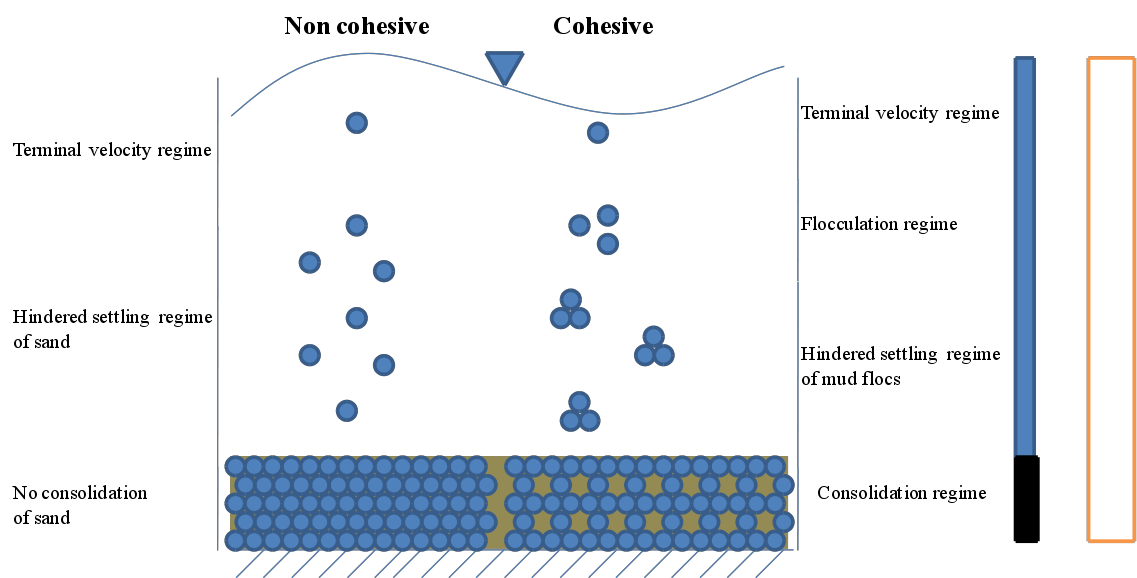
\includegraphics[scale=0.30,angle=0]{graphics/fig3.png}
\caption{Diagram of different processes involved in the settling transport
(left: non-cohesive, right : cohesive).}\label{fig:3}
\end{center}
\end{figure}

\subsection{Multi-layer empirical algorithm}\label{sec:4.2}

\subsubsection*{Time evolution}

The consolidation effect is reproduced by assuming that the vertical flux of
sediment from layer $j$ to underneath layer $j+1$ is proportional to the mass of
sediments, $M_s$ (kg/m2), contained in the layer $j$.

\begin{equation}\label{eq:eq8}
\frac{dM_s(j)}{dt} = a_i M_s(j) 
\end{equation}

The transfer mass coefficients $a_j$ (in s$^{-1}$) are specified in the
steering file (\texttt{MASS TRANSFER PER LAYER}). They correspond to a
characteristic timescale to transfer mass from one layer to another.

This multilayer consolidation model is not related to Gibson equation so
that it should be considered as empirical. Despite its apparent simplicity,
it can qualitatively reproduce an increase of mud bed deposit with time,
while ensuring mass conservation (transfer coefficient of the last bottom
layer is zero). The model results are highly sensitive to the specified
values of the mass transfer coefficients $a_i$ which are however difficult
to calibrate. The main advantage of this iso-pycnal formulation relies in
the fact that no vertical grid is required to compute the concentration
evolution of the different layers.

\subsubsection*{Discretization}

The vertical resolution of semi-empirical equation~\ref{eq:eq8} is based on the
multi-layer iso-pycnal model with fixed concentrations. The consolidation is
then reproduced by mass transfer between layers of the model. The transfer
coefficients are fixed for each layer.

The set of mass-transfer coefficients $a(j)$ in (s$^{-1}$) are selected by
calibration, in order to find best agreement of time-varying concentration
profiles between model and experiment. Physically, they represent the
inverse of the residence time per layer. The values $a(j)$ are found to
decrease from top to bottom, as the time scale of consolidation (or
residence time) increases. The mass transfer of the last layer is set to
zero, in order to insure no mass loss at the rigid bed level (impermeability
condition).

\medskip
\begin{bclogo}[couleur=blue!10,arrondi=0.1, logo=\bcinfo]{Keywords}
\begin{itemize}
\item {\ttfamily COHESIVE SEDIMENT = YES} ({\ttfamily = NO}, default option)
\item {\ttfamily MUD CONSOLIDATION = YES} ({\ttfamily = NO}, default option)
\item {\ttfamily CONSOLIDATION MODEL = 1} 
\item {\ttfamily NUMBER OF LAYERS OF THE CONSOLIDATION MODEL} ({\ttfamily NOMBLAY=10} by default, maximum value is 20 )
\item {\ttfamily MUD CONCENTRATION PER LAYER} (in kg/m$^3$, $E= 50.; 100.;...$ by default)
\item {\ttfamily MASS TRANSFER PER LAYER} ($= 5.0E-5,...,0.$, by default)
\end{itemize}
\end{bclogo}

\subsection{Multi-layer iso-pycnal Gibson's model}\label{sec:4.3}

\subsubsection{Theoretical background}

The previous equation presents the advantage of not using a vertical mesh.
However it is not physically based model since it neglects the Gibson
theory. Improvement of this category of model was proposed by Sanchez (1992)
and Thiebot (2008). In these formulations, the sediment flux from one layer
to the other is given not in term of empirical mass transfer coefficient ($a_i$) 
but in term of theoretical flux which is given by the Gibson theory.

\subsubsection{Numerical discretization}

The model originally developed by Sanchez (1992) and Thiebot
(2008) is a 1DV sedimentation-consolidation multi-layer model, based on an original
technique to solve Gibson equation. The advantage of this representation
(Equation~\ref{eq:eq9a}) if compared with previous one (Equation~\ref{eq:eq8}) relies on the right hand side term
which relates the mass of sediments, $Ms_i$ (kg), to the net flux entering
or leaving the layer. This equation enables therefore to consider the flux
of sedimentation and consolidation as provided by the Gibson theory.

\begin{equation}\label{eq:eq9a}
\dfrac{d Ms_i}{dt} = (F_i(t) - F_{i+1}(t))\Delta t \pi r^2 
\end{equation}%

In Equation~\ref{eq:eq9a}, a circular shape (of radius $r$) is assumed for the surface.
Equivalently, Equation~\ref{eq:eq9b} is expressed in term of layer thickness $Es_i$ (m), 
recalling $Ms_{i}$= Cs$_{i}$ $\pi$r$^{2}$ Es$_{i}$$_{.}$. This
last expression becomes independent on the settling column geometry.

\begin{equation}\label{eq:eq9b}
\dfrac{dEs_i}{dt} = \dfrac{F_i(t) - F_{i+1}(t)}{Cs_i} 
\end{equation}%

The concentration of the different bed layers $Cs(i)$ is fixed. As the
sedimentation and consolidation progress, the sediment is transferred to the
more concentrated layers, and the thickness of these layers increase as well.

\begin{figure}[H]
\begin{center}
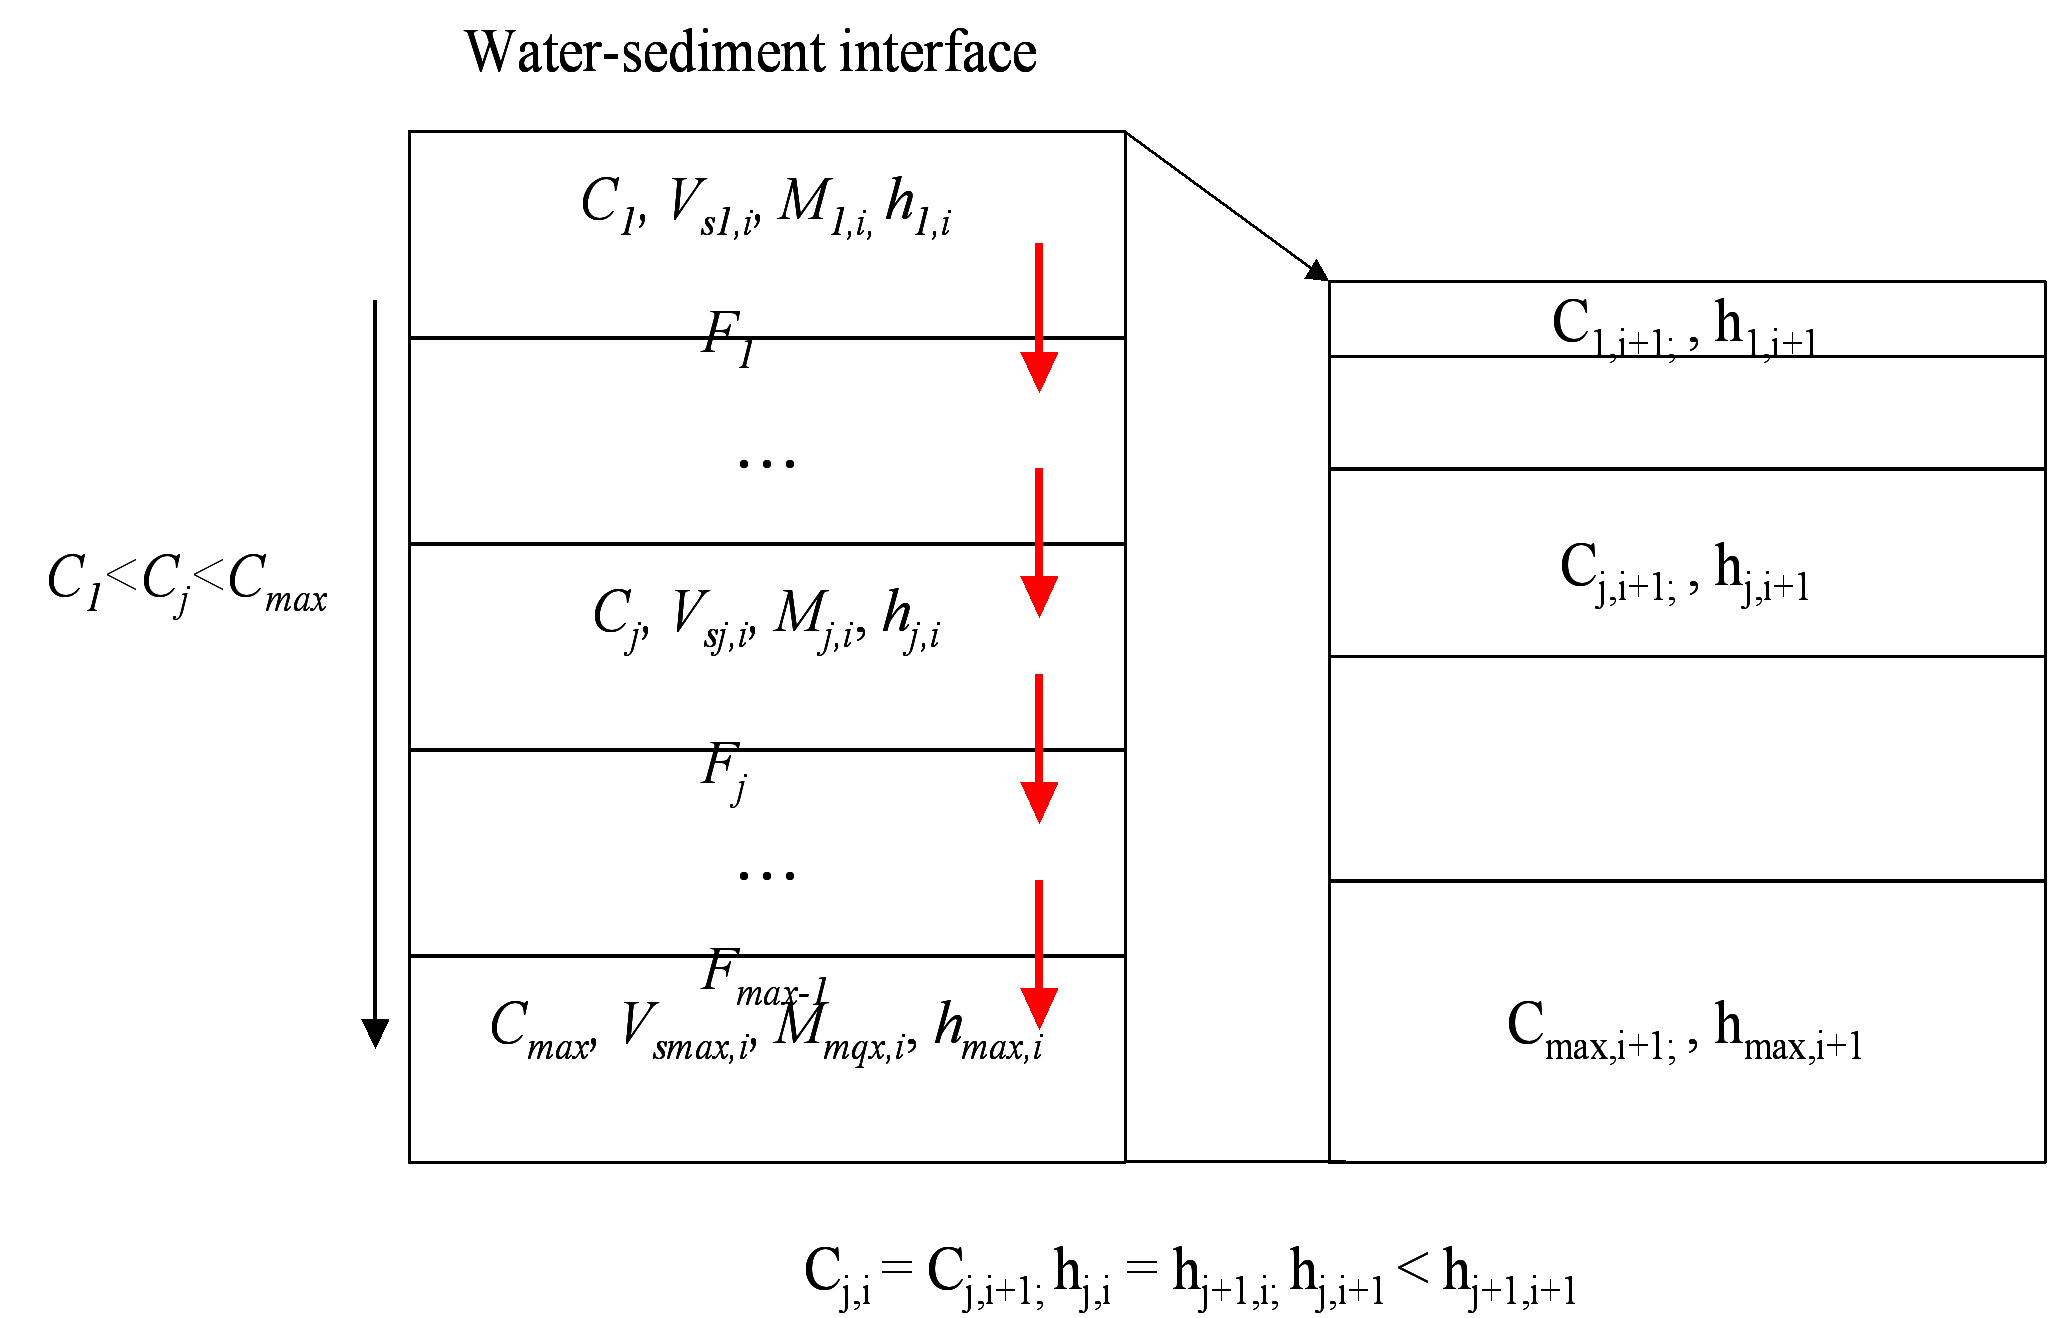
\includegraphics[scale=0.075,angle=0]{graphics/figNEW.png}
\end{center}
\end{figure}

The mass conservation is ensured by requiring at each moment, in each layer, the
equality between the mass contained in a layer at time $t + \Delta t$ and the
mass present in this layer at time $t$ in which the outgoing mass was removed
and the incoming mass was added (means the mass that crossed the upper and
lower sections respectively during the time $\Delta t$). The outgoing and
incoming masses are taken into account by sediment flux noted $F_i(t)$.

\begin{equation}
F_i(t) = \dfrac{(V_{s,i}(t) -V_{s,i-1}(t))C_{i-1} C_i}{C_{i-1} - C_i} 
\end{equation}

where $V_{s,i}$ is the falling velocity of the layer $i$, and can be
defined as:

\begin{equation}
V_{s,i}(C_i) =\left\{\begin{array}{ll}
k(C_i)C_i\left(\dfrac{1}{\rho_s} - 
\dfrac{1}{\rho_f} \right), & \quad\text{if}\,C_i \leq C_{gel}\\
k(C_i)C_i \left(\dfrac{1}{\rho_s} -\dfrac{1}{\rho_f} \right) 
+ k(C_i)\dfrac{\sigma'(C_{i-1})-\sigma'(C_{i} )}{\dfrac{1}{2}(Ep_{i-1}(t)+Ep_i(t))}, & \quad\text{otherwise}
\end{array}
\right.
\end{equation}

where $k$ is the permeability, $\sigma'$ is the effective stress, $C_{gel}$ 
the transition concentration between sedimentation and consolidation
schemes (Camenen \& Pham Van Bang, 2011). The closure equation is presented
in section~\ref{sec:4.5}.

\subsection{Vertical grid Gibson's model}\label{sec:4.4}
Vertical-grid models propose a natural resolution of the Gibson equation
as a vertical grid is used to compute the concentration at each point. This
category of model uses common techniques (finite difference or finite volume
or finite element methods) for resolving partial differential equations.

As they use a vertical grid, the connection with \sisyphe which is depth
integrated model is not straightforward.

In the new version of \sisyphe, such a category of model is also available.
Strictly speaking, the original Gibson model (in material coordinate) used
in \telddd which was developed by Lenormant (1993) is connected to
\sisyphe.

The finite difference method is used. The implicit scheme leads to a
tridiagonal matrix that is solved by using a classical double sweep
algorithm. More details are given in \telddd user guide, Lenormant
(1993) and Lan Anh Van (2012).



\section{Initialization and boundary conditions}

\subsection{Initial conditions}
The initial concentration for the suspended load can be either imposed
within \texttt{condim\_susp.f} or specified in the steering file through the keyword
\texttt{INITIAL SUSPENSION CONCENTRATIONS} initializes the value of the volume
concentration for each class.

The initial layer thicknesses are specified in user-subroutine
\texttt{init\_compo\_coh.f}. It is called by subroutine \texttt{init\_mixte.f} which just checks
if the sum of all layers is equal to the total bed thickness as specified by
the initial bathymetry $Z_f$ and rigid bed $Z_r$ :
%ICI REF (\ref{eq_test}) :

\begin{equation}\label{eq_test}
Z_f(i) - Z_r(i) = \sum_{j=1,NCOUCH\_TASS}E_s(i,j) 
\end{equation}
where $i$ is the number of point, $j$ the number of layer, $Z_f$ the bed level and $Z_r$ the non-erodible bed level.

\subsection{Boundary conditions}
For the boundary conditions, the concentration of each class can be
specified in the steering file through keyword \texttt{CONCENTRATION PER CLASS AT
BOUNDARIES}. It may be also convenient to use keyword \texttt{EQUILIBRIUM INFLOW
CONCENTRATION =YES}, the concentration at the entrance of the domain and at
$t=0$ is set to its equilibrium value, according to the choice of the
\texttt{REFERENCE CONCENTRATION FORMULA}. Input concentrations can be also directly
specified (user subroutines \texttt{conlit.f}).

\subsection{Equilibrium conditions}
The concentrations at the entrance of the domain can be calculated by
\sisyphe assuming equilibrium conditions in order to avoid unwanted
bed-evolution at the entrance of the domain, and also at the first time
step, it is possible to impose the concentration to its equilibrium value,
by activating the keyword \texttt{EQUILIBRIUM INFLOW CONCENTRATION}.

The equilibrium (depth-averaged) concentration is then calculated assuming
equilibrium concentration at the bed and a Rouse profile correction for the
$F$ factor.

\medskip
\begin{bclogo}[couleur=blue!10,arrondi=0.1, logo=\bcinfo]{Keywords}
\begin{itemize}
\item {\ttfamily INITIAL SUSPENSION CONCENTRATIONS} ($C_{S0} = 0$,
default value)
\item {\ttfamily EQUILIBRIUM INFLOW CONCENTRATION} (\texttt{= NO}, default value)
\item {\ttfamily CONCENTRATION PER CLASS AT BOUNDARIES} ($=0$, default value)
\end{itemize}
\end{bclogo}

\section{User subroutines}

The subroutine \texttt{condim\_susp.f} can be used to specify the initial conditions
for the sediment concentration (see {\S } V.4.2). 
The subroutine \texttt{conlit.f} can be used to specify the concentration at the
entrance of the domain.

%\section{Keywords}

\section{Application Test Cases}

\subsubsection{Erosion/deposition experiments}

\subsubsection{Description of experiments}

This part can be issued from the simulation of Aachen test cases on Gironde
mud. The description of the experiment, test results and simulation results
are fully detailed in Lan Anh Van (2012). This study has been published in
the 6th International Conference on Scour Erosion (Paris, August 27-31,
2012). This paper is available from the opentelemac website.

The annular flume at Aachen University (Germany) is used to imposed stepwise
increase (erosion test) and stepwise decrease (deposition test) of bottom
shear stress on cohesive bed. Figure \ref{fig:4} presents the hydraulic facility and
describes the forcing. The Gironde mud is used as cohesive sediment. The bed
is initially prepared at $300$ g/L.

\begin{figure}[H]
\begin{center}
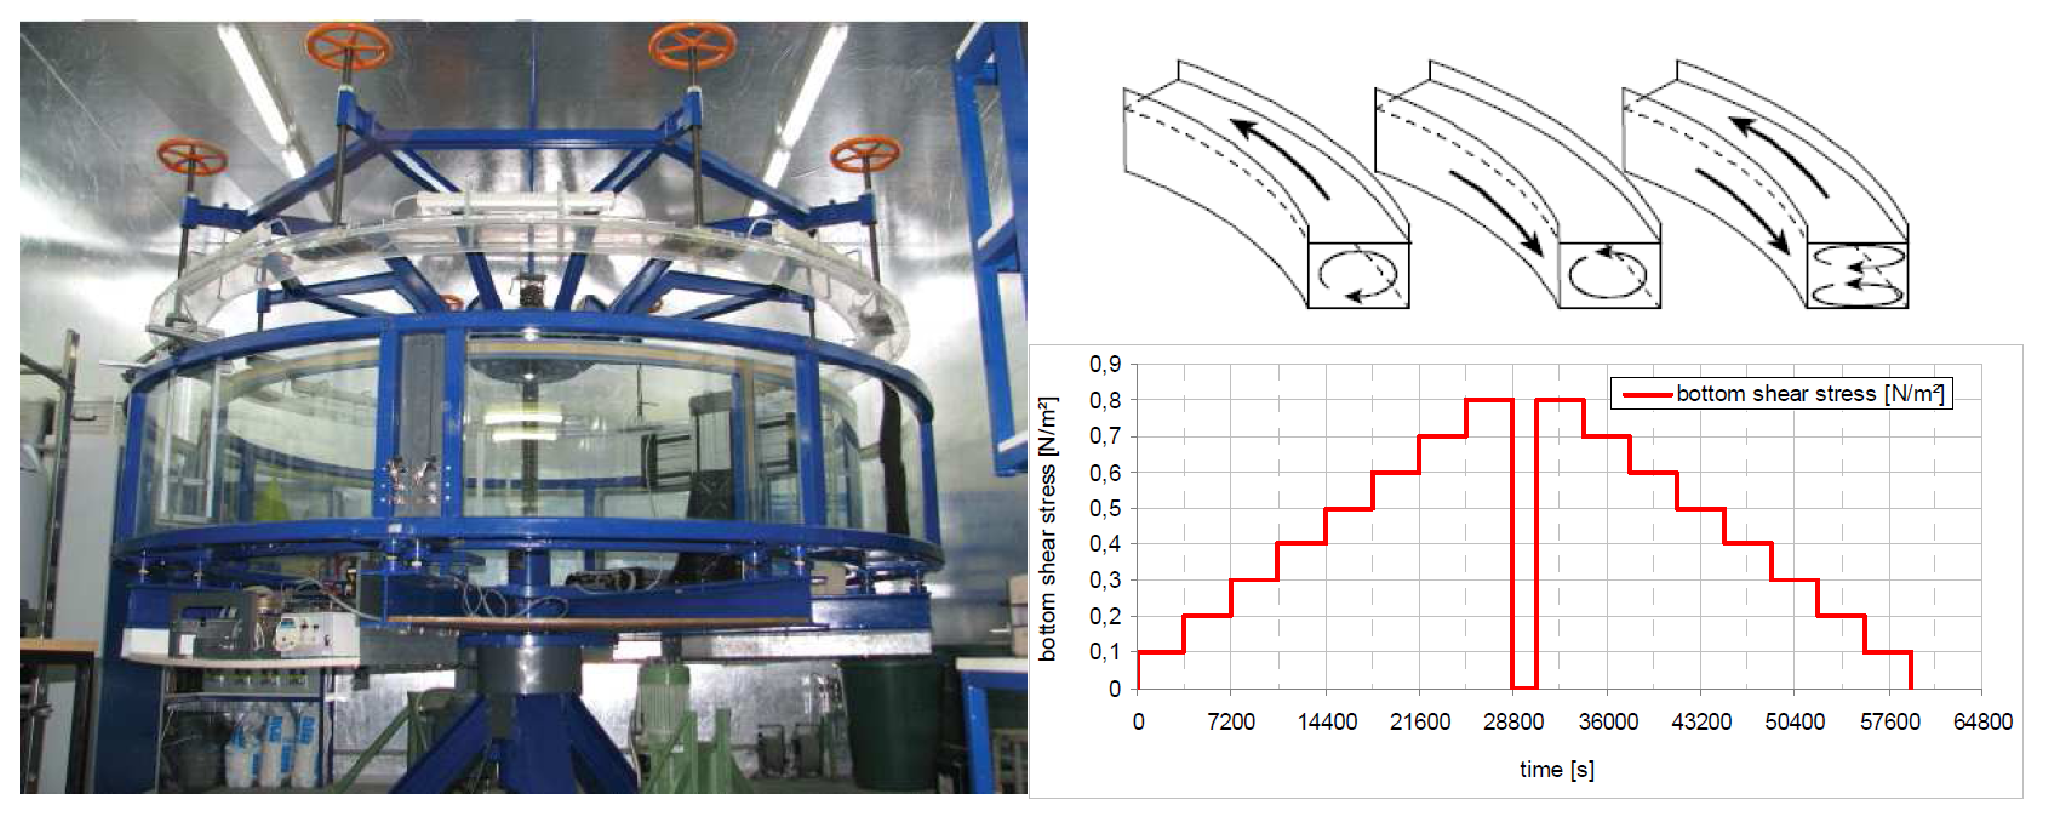
\includegraphics[scale=0.25,angle=0]{graphics/fig4.png}
\caption{Annular
flume (RWTH, Aachen, Germany) on the left, the middle figure shows the step
wise increase of bed shear stress during the erosion phase, while the figure
on the right hand side shows the decrease during the deposition phase.}\label{fig:4}
\end{center}
\end{figure}

\subsubsection{Erosion test}

In \sisyphe, we consider the hydraulic flume as straight in order to
simplify. The bed is modeled by four layers having increasing concentration.
The top layer (layer 1) has initial concentration of $150$ g/L and thickness
$0.4$ cm (see Table 1 below). The erosion parameters (critical shear stress $\tau_{*e}$ and kinetic parameter $M$) 
of the Partheniades law for the considered material (Gironde mud) of each layer is presented in the
Table. The value are obtained from best fitting exercice on the test results
which are presented in Figure~\ref{fig:5} with the simulation results. 

\begin{table}
\begin{center}
   \caption{\label{tab:1} Example
of cohesive sediment bed composition}
\begin{tabular}{|c|c|c|c|c|}
  \hline
  Layer & Concentration (g/l) & Thickness (cm) & $\tau_{*e}$ (N/m$^2$) & $M$ (kg/m$^2$/s) \\
  \hline
  1 & 150 & 0.40 & 0.10 & 1.86$\times 10^{-3}$\\
  2 & 200 & 0.70 & 0.22 & 4.4$\times 10^{-3}$ \\
  3 & 250 & 0.40 & 0.35 & 8.0$\times 10^{-3}$\\
  4 & 300 & 2.50 & 0.47 & 0.132\\
  \hline
\end{tabular}
\end{center}
\end{table}

\begin{figure}[H]
\begin{center}
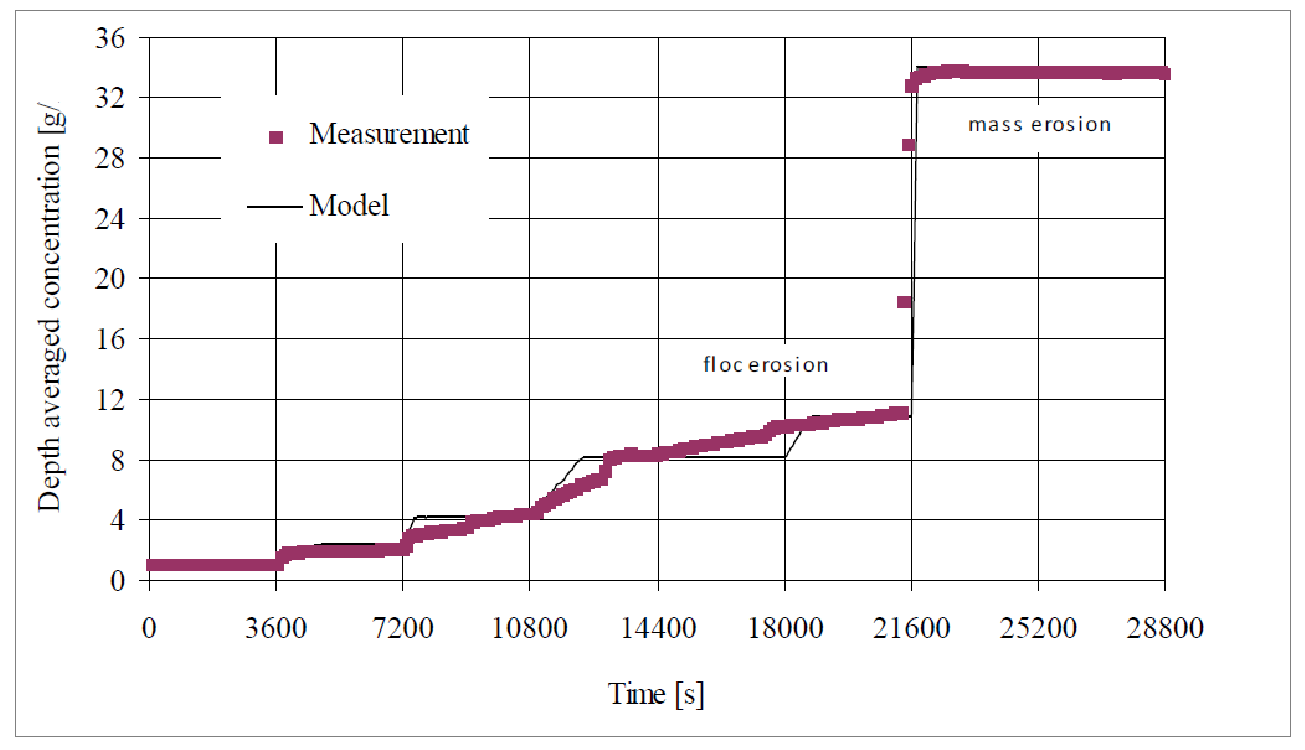
\includegraphics[scale=0.35,angle=0]{graphics/fig5.png}
\caption{Comparison between modelled and measured concentration during the erosion
phase.}\label{fig:5}
\end{center}
\end{figure}

Since erosion parameters differ from one layer to the other, both erosion
processes, the floc erosion and the mass erosion, can be reproduced.
Regarding the test results, a minimal number of four layer is required for
the simulation exercice. 

\subsubsection{Deposition test}

After the stepwise increase of the bottom shear stress, the decreasing phase
(or deposition test) takes place during the experiment. The sediment bed is
fully eroded: all the sediment are transported as suspension having a depth
averaged concentration equal to $33.8$ g/L. From the test results on
deposition tests, the critical deposition velocity, $u_{*d}$, is measured as
equal to $0.016$ m/s. And the measurement from Owen tube provides the
relationship between the settling velocity $W_s$ and the concentration $C$:

\begin{equation*}
W_s (mm/s)=\left\{ 
\begin{array}{cl}
0.15C^{2.1} & \quad \text{if}\quad C < 4.5 g/L \\ 
3.5 & \quad \text{if}\quad C > 4.5g/L
\end{array}
\right. 
\end{equation*}

Figure 6 illustrates the agreement between experiment and simulation which
is obtained from the formula by Krone (Equation~\ref{}) and the parameter values
described previously. 

\begin{figure}[H]
\begin{center}
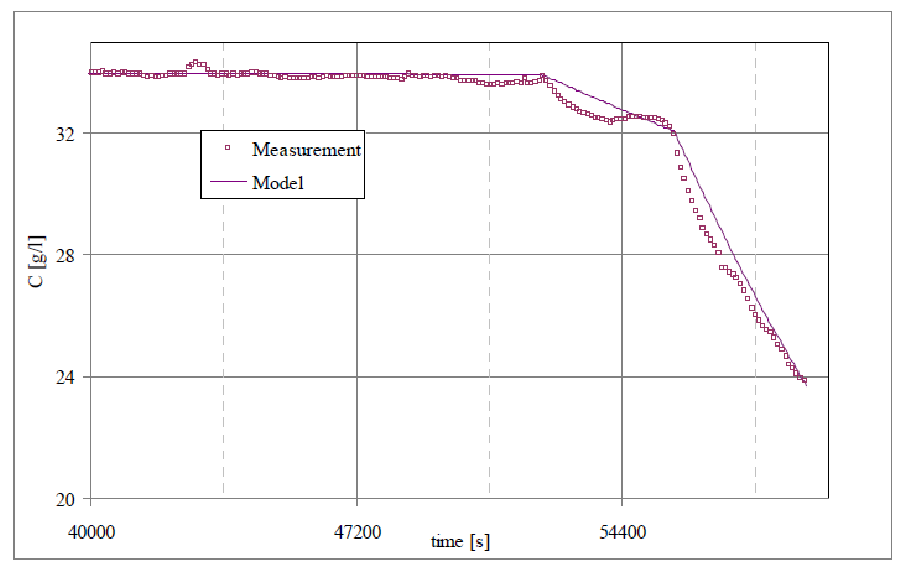
\includegraphics[scale=0.45,angle=0]{graphics/fig6.png}
\caption{Comparison between modelled and measured concentration during the deposition
phase.}\label{fig:6}
\end{center}
\end{figure}

\newpage

\subsubsection{Consolidation tests}
The different consolidation models developed in \sisyphe have been validated
against measurements made by Lan Anh Van (2012) in a settling column. In
this part we will present the experimental device (X-ray) used to obtain
space-time resolved data on the process. This test case is available as a
reference test in release 6.3.

\subsubsection*{Data set}
Gironde mud is tested in a settling column which is instrumented by X-ray
technique. The prototype was initially developed at the Commissariat \`{a}
l'Energie Atomique (CEA, Saclay, France) and improved for this study at
Chatou. The final version of the prototype is illustrated in Figure~\ref{fig:7}. More
details on the measuring principle (attenuation of signal or
transmitometry), the calibration procedure (Beer-Lambert law), the
experimental conditions of testing (initial homogeneous sample) are
available in Lan Anh Van (2012).

\begin{figure}[H]
\begin{center}
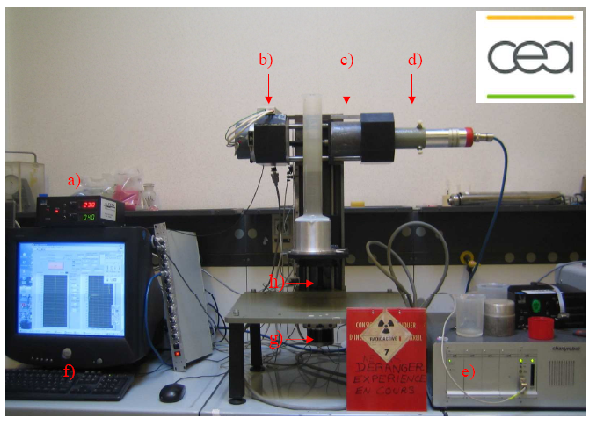
\includegraphics[scale=0.55,angle=0]{graphics/fig7.png}
\caption{X-ray settling column device (CEA/DRT/LIST, Saclay): a) supply of the X-Ray generator; b) X-Ray generator; 
c) collimator (5mm slot); d) photon detector; e) computer controlled unit; f) acquisition
data unit; g) step motor; h) endless screw.}\label{fig:7}
\end{center}
\end{figure}

\begin{figure}[H]
\begin{center}
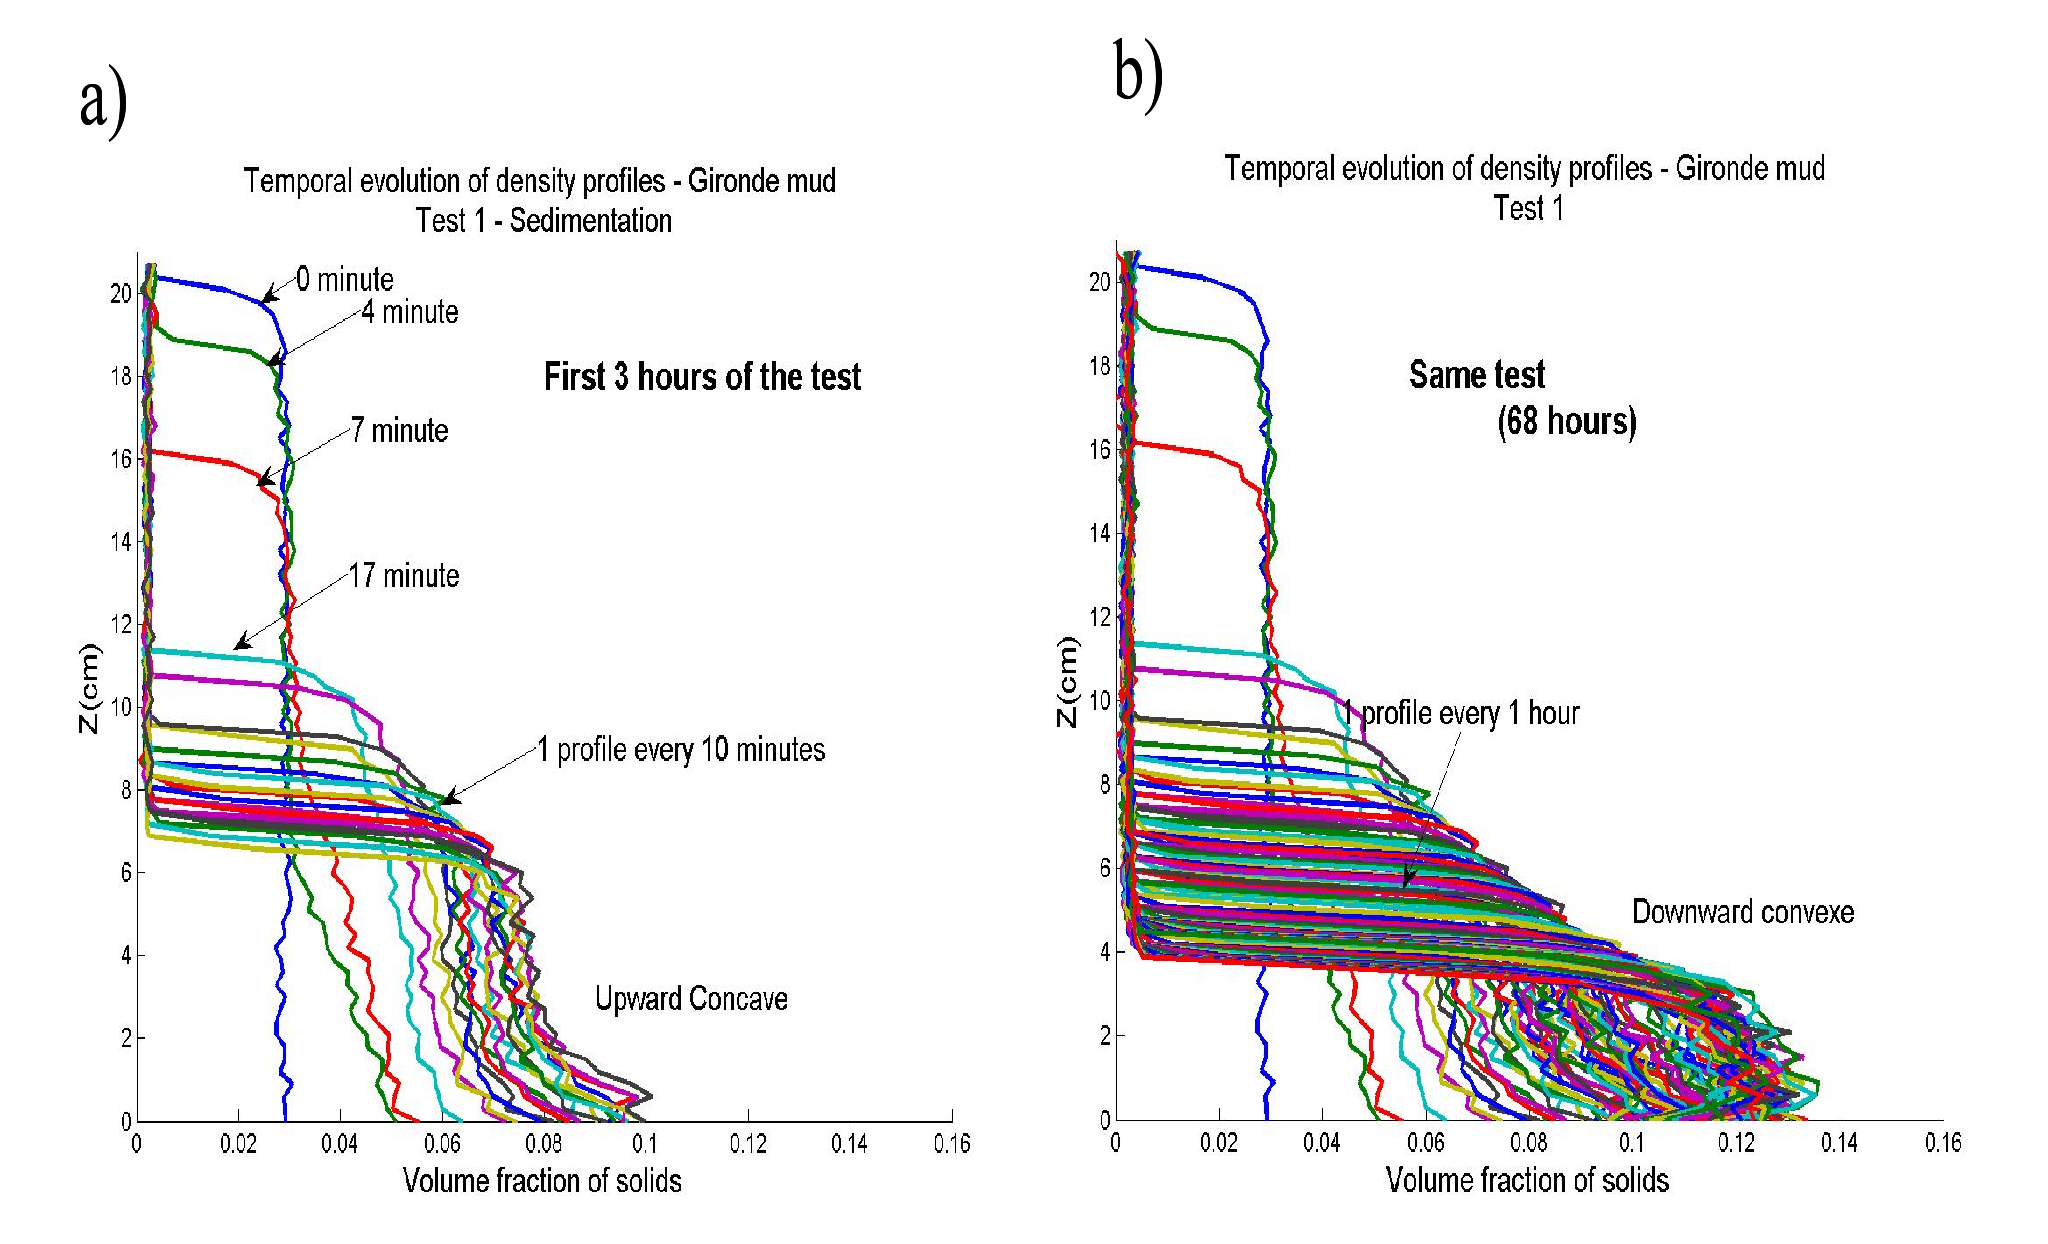
\includegraphics[scale=0.1,angle=0]{graphics/fig8.png}
\caption{time evolution of concentration profile during the
sedimentation-consolidation of Gironde mud. The settling column is 20.7cm
height, the suspension was initially prepared at solid fraction equal to
2.96\% (Villaret et al. 2010).}\label{fig:8}
\end{center}
\end{figure}

Figure 8 (left, first 3 hours of the test) presents concentration (vertical)
profiles having an upward convex shape near the bottom. This shape becomes
downward convex in Figure 8 (right, long term). This difference is explained
by the different nature of the governing process (See L.A. Van, 2012). At
short term, the hindered settling (convection term) is the governing
process. For moderate concentration (sufficiently far from the gelling
point), the upward convex shape is obtained if we consider the
Richardson-Zaki law. At long term and large concentration (larger than the
gelling point), the consolidation (diffusion term) is dominant. As a
consequence, the near bottom concentration profile becomes downward convex.%

\subsubsection*{Model 1}
The multi-layer empirical algorithm initially developed by Walther \&
Villaret (2008) is used on the data presented by Figure~\ref{fig:8}. Here $20$ layers
were used to model the vertical profile of concentration. Table~\ref{tab:2} presents
the model parameters (mass transfer coefficient $ai$) which are adjusted on
data for best agreement.

\begin{table}
\begin{center}
   \caption{\label{tab:2} Calibrated parameters of Model 1}
\begin{tabular}{|c|c|c|c|c|c|c|c|c|c|c|}
  \hline
Layer  & 1 & 2 & 3 & 4 & 5 & 6 & 7 & 8 & 9 & 10 \\  
  \hline
coef. $a$ & 1$\times 10^{-2}$ & 8$\times 10^{-3}$ & 6$\times 10^{-3}$ & 4$\times 10^{-3}$ & 2$\times 10^{-3}$ & 1$\times 10^{-3}$ & 8$\times 10^{-4}$ & 6$\times 10^{-4}$ & 4$\times 10^{-4}$ & 2$\times 10^{-4}$ \\
  \hline
Layer  & 11 & 12 & 13 & 14 & 15 & 16 & 17 & 18 & 19 & 20 \\
 \hline
coef. $a$ & 1$\times 10^{-4}$ & 8$\times 10^{-5}$ & 6$\times 10^{-5}$ & 4$\times 10^{-5}$ & 2$\times 10^{-5}$ & 1$\times 10^{-5}$ & 1$\times 10^{-5}$ & 1$\times 10^{-5}$ & 1$\times 10^{-5}$ & 0 \\
  \hline  
\end{tabular}
\end{center}
\end{table}

Figure 9 presents the simulation results by using the multi-layer empirical
approach with the parameters given in Table 2.\newline

\begin{figure}[H]
\begin{center}
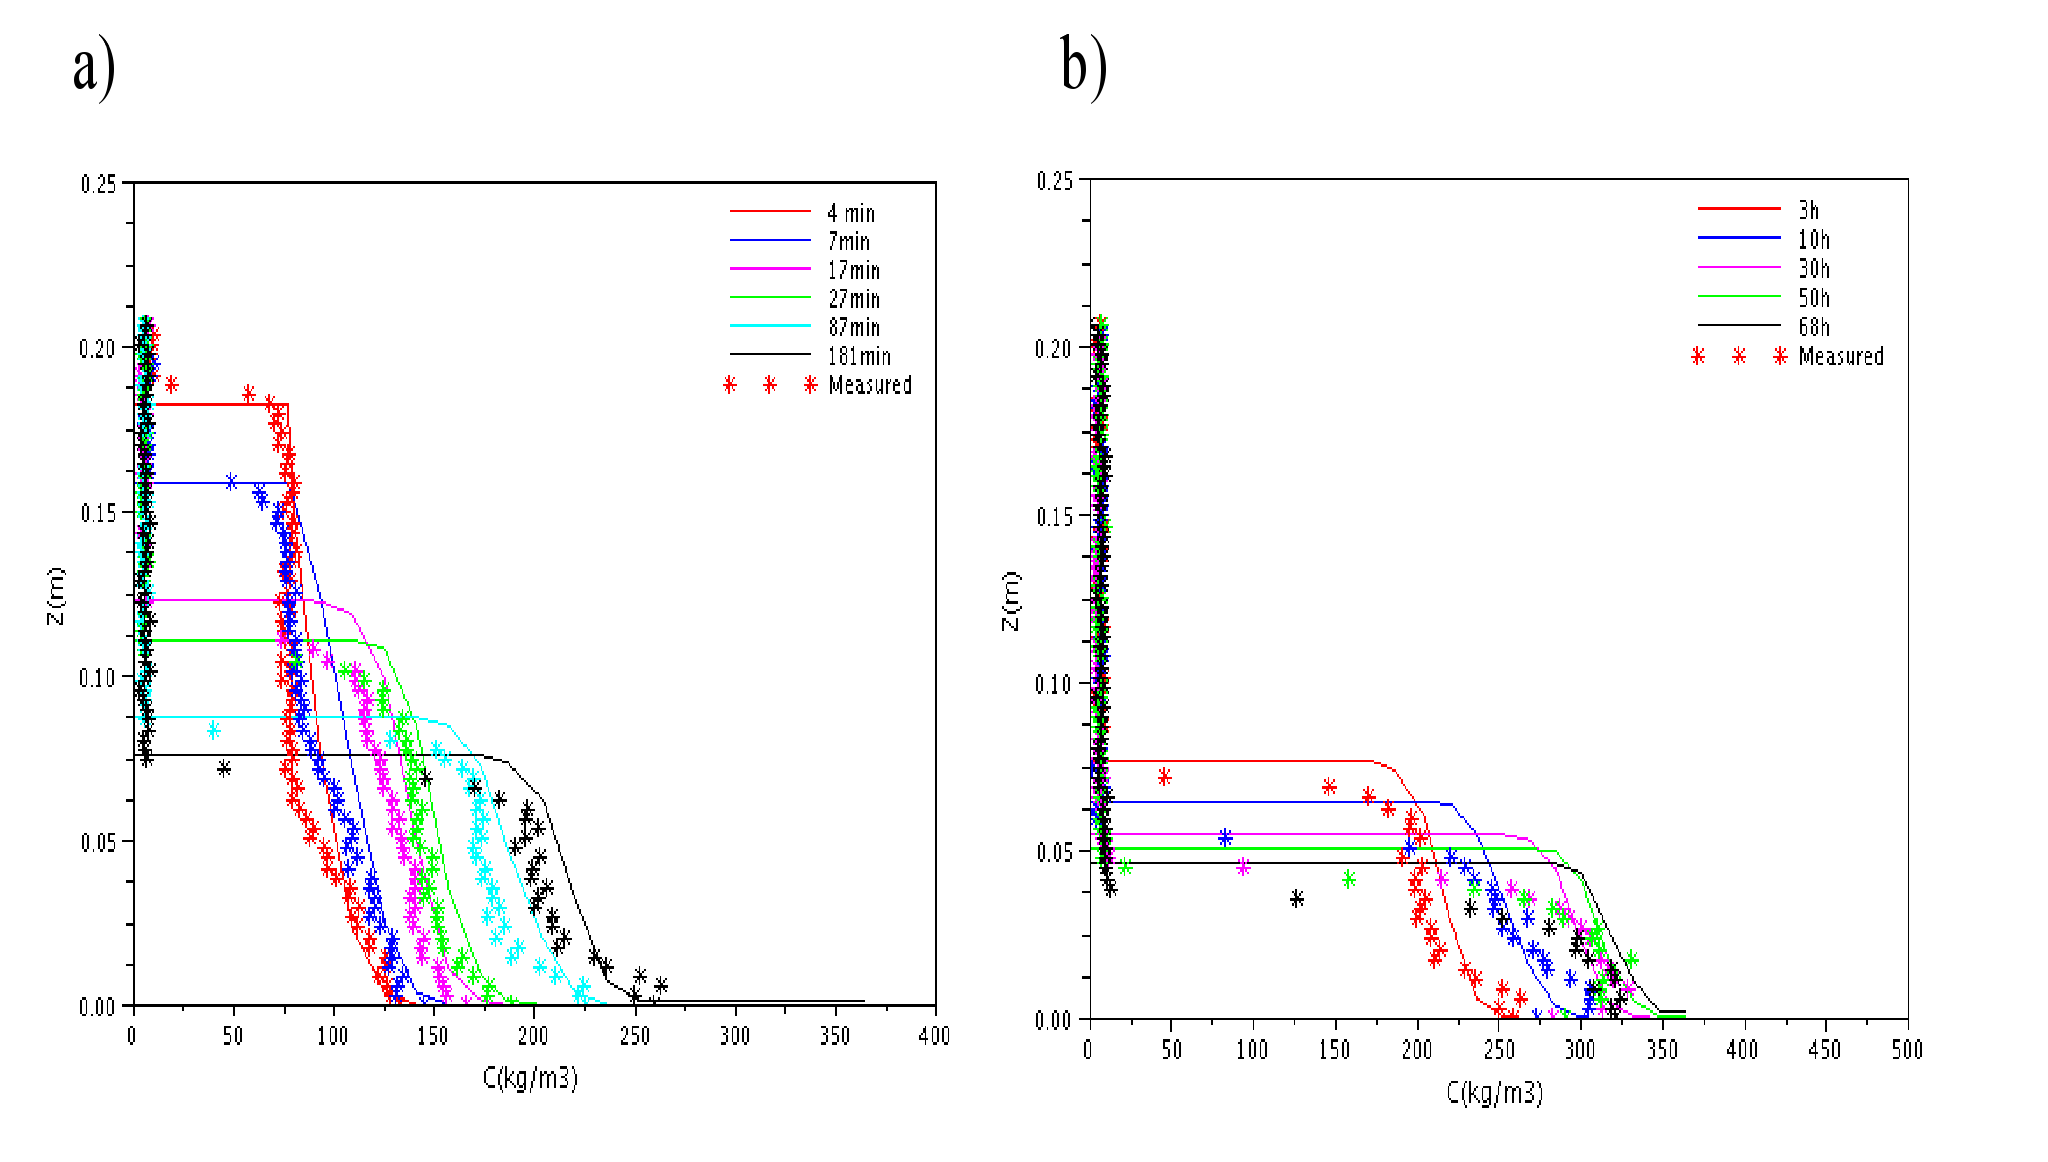
\includegraphics[scale=0.1,angle=0]{graphics/fig9.png}
\caption{Simulation results from multi-layer empirical approach : a)
sedimentation; b) consolidation.}\label{fig:9}
\end{center}
\end{figure}

\subsubsection*{Model 2}
Model 2 (multi layer iso-pycnal Gibson model, see~\ref{sec:4.3}) and vertical grid
Gibson model, see \ref{sec:4.4} are more rigorously based on Gibson theory than
previous Model 1. The space-time methodology for the determination of
closure equation and parameters is therefore enabled.

Application of the space-time procedure (see~\ref{sec:4.5}) provides the closure
equations with parameters which are presented in the following table. From
isoconcentration (straight) lines, slopes are measured which correspond to
the first derivative of the solid flux. Integration of this last result
provides the solid flux and consequently the hindered settling velocity.

\begin{figure}[H]
\begin{center}
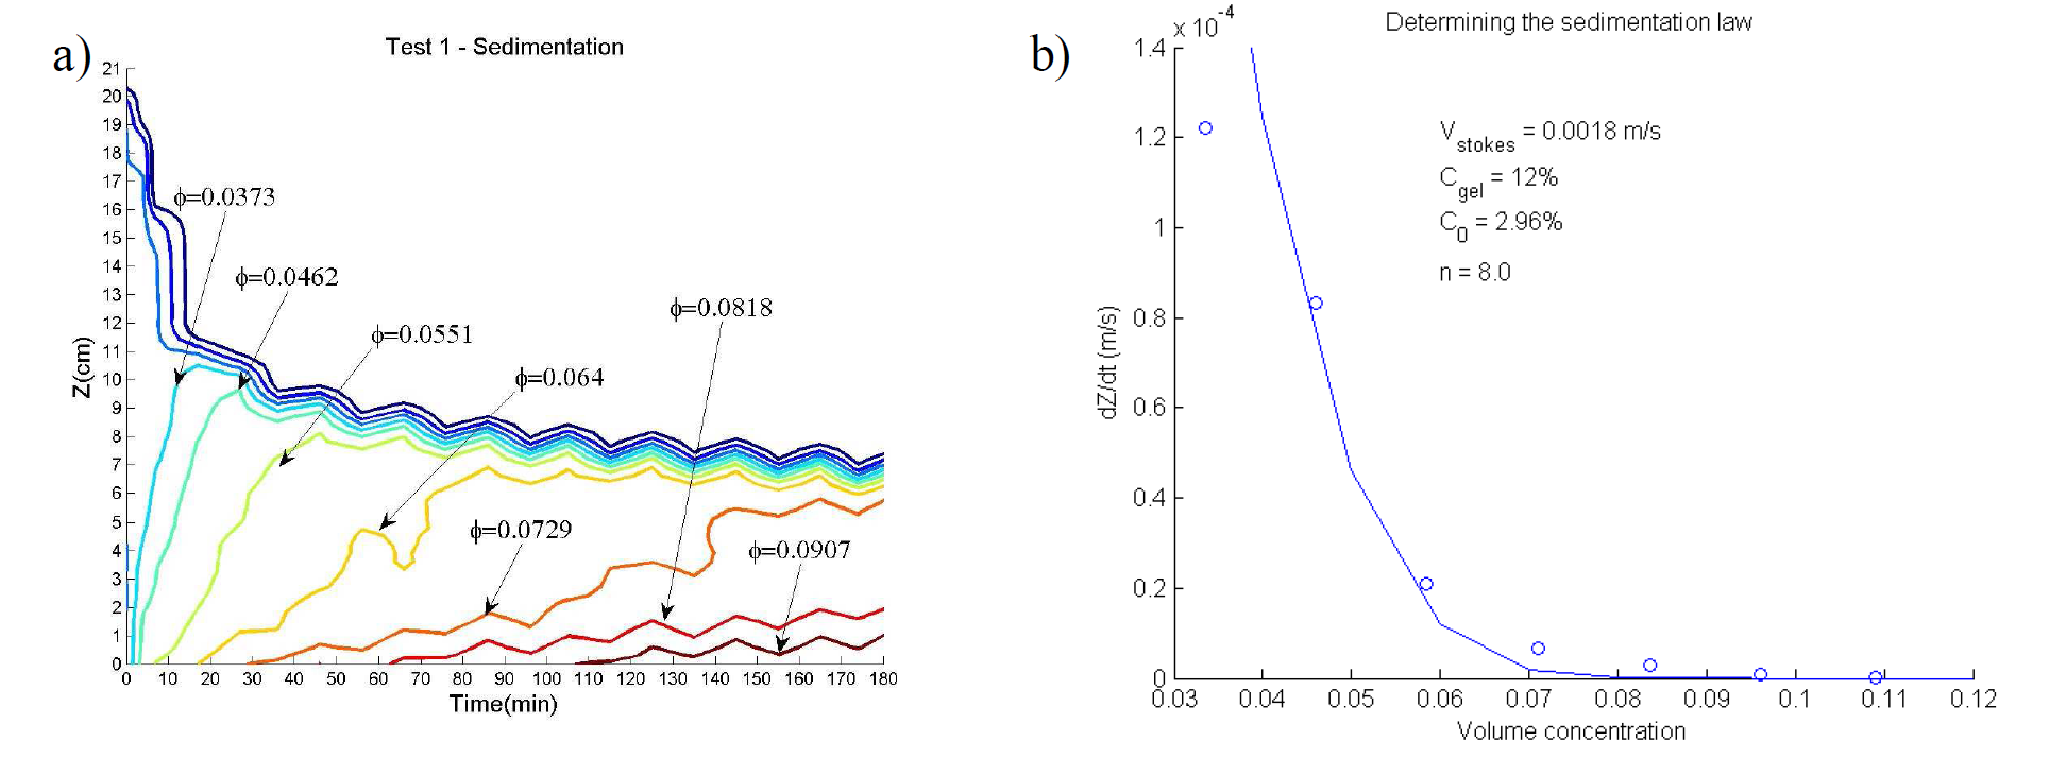
\includegraphics[scale=0.2,angle=0]{graphics/fig10.png}
\caption{Determination of the hindered settling flux $f$ (Eq. 16).}\label{fig:10}
\end{center}
\end{figure}

\begin{figure}[H]
\begin{center}
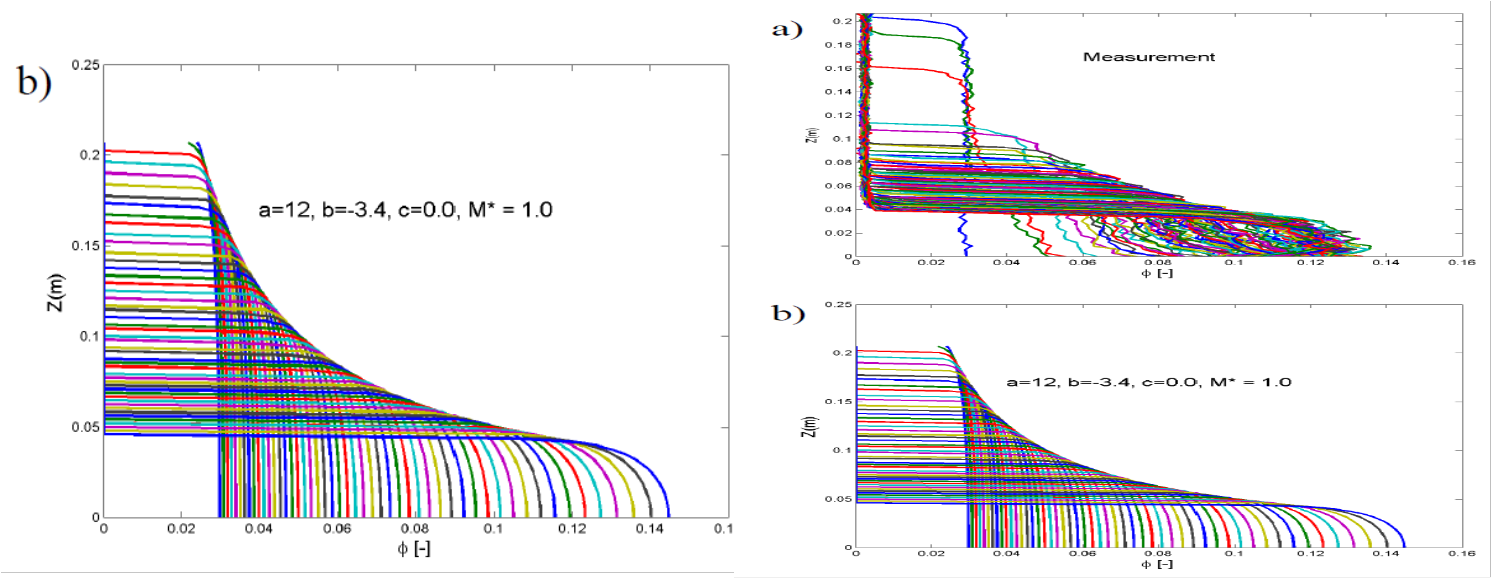
\includegraphics[scale=0.35,angle=0]{graphics/fig11.png}
\caption{Determination of the consolidation (concentration and time dependent non
linear diffusion) parameters used in the similarity solution $h$ (Eq. 18).}\label{fig:11}
\end{center}
\end{figure}

The space-time new methodology applied to the test case on Gironde mud leads
to the calibration results (Table~\ref{tab:3}).


\begin{table}
\begin{center}
   \caption{\label{tab:3} Parameters of Models 2 and 3}
\begin{tabular}{|l|c|c|}
  \hline
Model & Model 2 & Model 3 \\
 \hline
closure equation & $k(C)=\dfrac{V_{st}}{s-1} (1-\dfrac{C}{\rho_s} )\left(1-\dfrac{C}{
C_{gel}}\right)^n\dfrac{\rho_s}{C}$ & $k(e)=\dfrac{V_{st}}{s-1}\left(\dfrac{e}{1+e}\right)\left(\dfrac{
e-e_{gel}}{1+e}\right)^n$ \\
for $k$ for $C<C_{gel}$  &  & \\
  \hline  
closure equation & $k(C)=\dfrac{V_{st}}{s-1} (1-\dfrac{C}{\rho_s} )\left(1-\dfrac{C}{
C_{max}}\right)^n\dfrac{\rho_s}{C}$ & $k(e)=\dfrac{V_{st}}{s-1}\left(\dfrac{e}{1+e}\right)\left(\dfrac{
e-e_{max}}{1+e}\right)^n$ \\
for $k$ for $C\geq C_{gel}$  &  & \\
  \hline  
closure equation & $\dfrac{\partial\sigma'}{\partial C} =-\left[11.55\left(\dfrac{C
}{C_0} \right)^{12} t^{-3.4}\right]\dfrac{\gamma_w}{kC}$ & $\dfrac{\partial\sigma'}{\partial e} =-\left[11.55\left(\dfrac{
1+e_0}{1+e}\right)^{12} t^{-3.4}\right]\dfrac{\gamma_w}{k/(1+e)}$ \\
for $\sigma'$ &  & \\
\hline 
$V_{stokes}$ (m/s) & 0.0018  & 0.0018 \\
\hline 
gel point & $C_{gel}=312$ g/l & $e=7.33$ \\
 \hline 
max concentration & $C_{max}=400$ g/l & $e_{max}=5.50$ \\
\hline
$n$ & 8 & 8 \\
\hline
\end{tabular}
\end{center}
\end{table}

We recall here that Model 2 (multi layer iso-pycnal Gibson's model) is
solving the problem in Eulerian coordinate and in mass concentration whilst
Model 3 (vertical grid Gibson's model) is concerning the same problem in
material coordinate (see Annexe 9.3 for the description of the
transformation between both system of coordinate) and in term of void ratio $e$. Indeed both models run with the same closure equation and parameter
values.

\begin{figure}[H]
\begin{center}
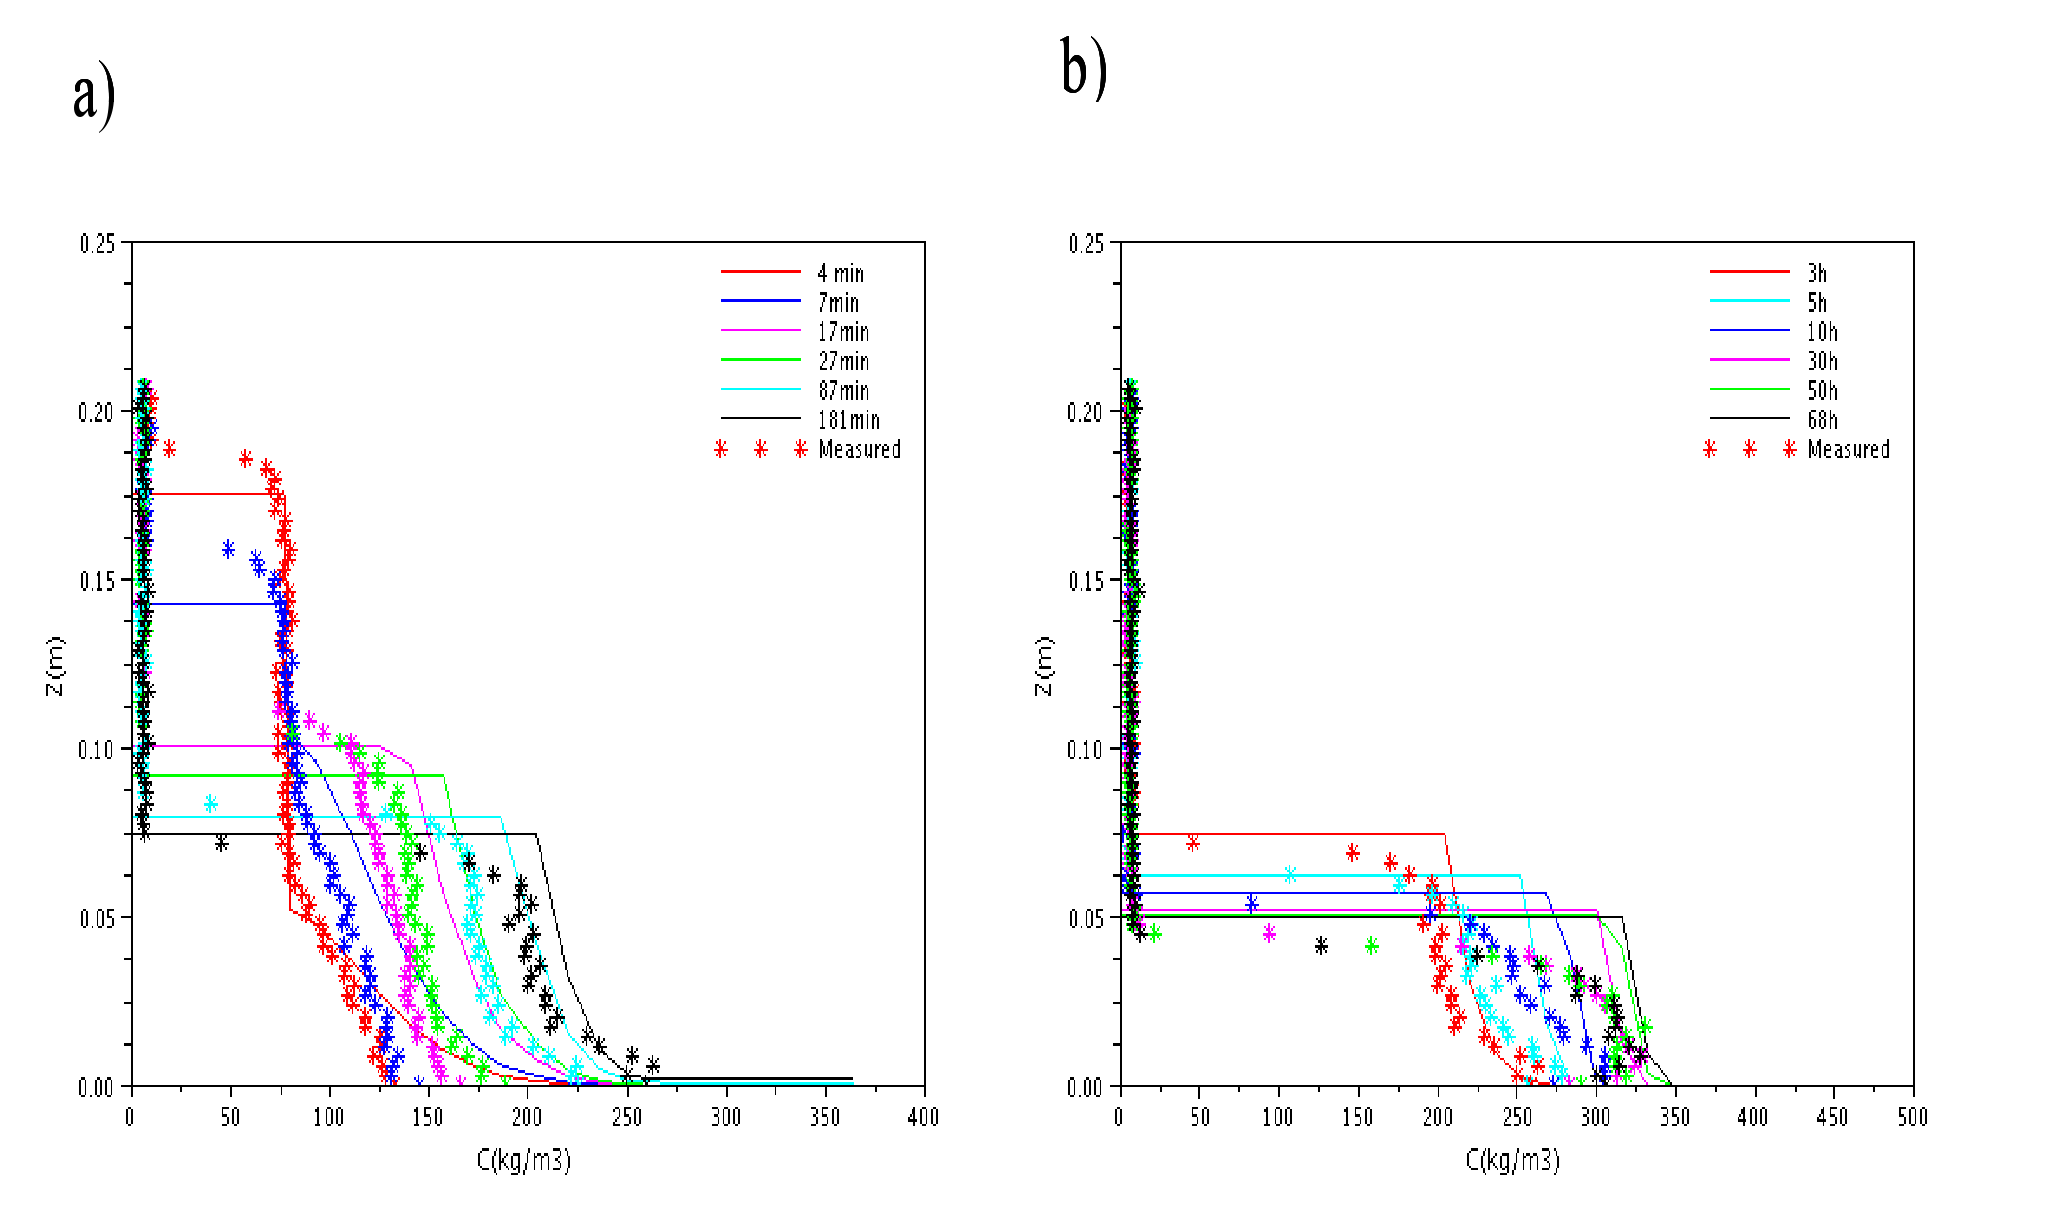
\includegraphics[scale=0.1,angle=0]{graphics/fig12.png}
\caption{Simulation results from multi-layer iso-pycnal Gibson model : a)
sedimentation; b) consolidation.}\label{fig:12}
\end{center}
\end{figure}

\subsubsection*{Model 3}

Both Models 2 and 3 use the same closure equations for the convection and
diffusion terms (Table 2.6). However, Model 3 is formulated in material
coordinate in term of void fraction $e$ whilst the Model 2 considers the
eulerian coordinate and the mass concentration. The coordinate and parameter
transforms are detailled in Appendix 9.3.

Figure 13 presents the simulation results from Model 3.

\begin{figure}[H]
\begin{center}
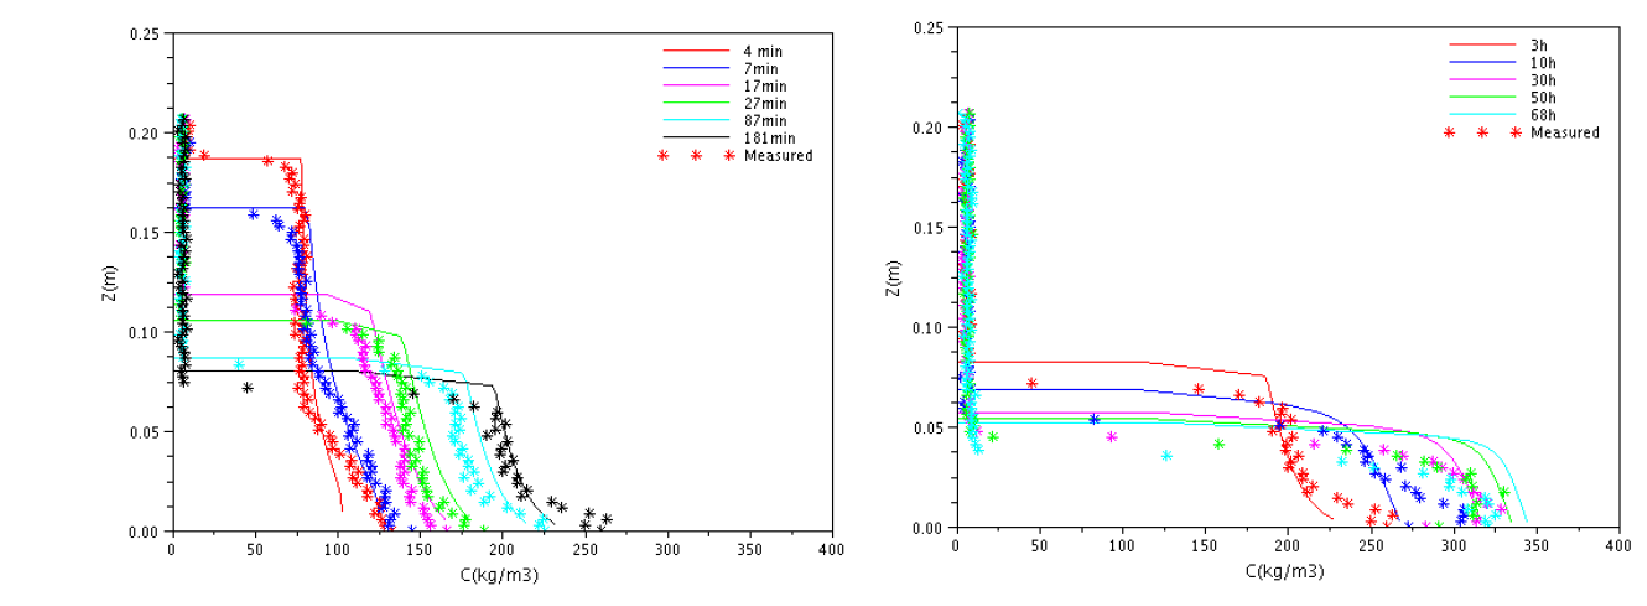
\includegraphics[scale=0.25,angle=0]{graphics/fig13.png}
\caption{simulation results from model 3 (vertical grid Gibson's model) with
parameters presented in Table 2.6.}\label{fig:13}
\end{center}
\end{figure}

\section{Appendix: Closure equations for permeability and effective stress}

All of the Gibson based models, i.e. Multi-layer iso-pycknal Gibson's model
(section~\ref{sec:4.3}) and vertical grid Gibson model (section~\ref{sec:4.4}), requires two
closure equations. The Multi-layer empirical model (section~\ref{sec:4.2}) only needs
closure on ai, the mass transfer coefficients.

In this section, some available empirical formula are detailed. In general,
a decreasing (or increasing) function of solid concentration is considered
for permeability $K$ (or effective solid stress). These expressions are
logarithmic or exponential or power law functions (see Bartholomeeusen et
al. 2002).

\subsubsection{Closure equations}
\begin{itemize}
\item Bed permeability $k$

Bartholomeeusen et al. (2002) introduced typical functions, in the form of
either power or exponential, to relate the permeability $k$ with the void
ratio $e$:

\begin{equation*}
k=\left\{\begin{array}{l}
A_1 e^{A_2} \\ 
A_1 \phi_s ^{-A_2 } \\ 
\exp (-A_1 +A_2 e)%
\end{array}
\right. 
\end{equation*}

The value of these coefficients $A_1$ and $A_2$ depend on grain size
distribution, organic content, activity and pore size distribution.

\item Effective stress $\sigma'$
The similar way can be opted in the determination of $\sigma'(e)$
($\sigma'(C),\sigma'(\phi)$), which gives:

\begin{equation*}
\left\{ 
\begin{array}{l}
e=-B_1 \sigma^{' B_2} + B_3 \\ 
\sigma' = B_1 \phi_s^{B_2} \\ 
\end{array}
\right. 
\end{equation*}%
or 
\begin{equation*}
\left\{ 
\begin{array}{l}
e=B_1 (\sigma'+ B_2)^{-B_3} \\ 
\sigma'=\exp (B_4+B_5 e)
\end{array}
\right. 
\end{equation*}%

According to Winterwerp \& van Kesteren (2004), the validity range of the
power-type functions (e.g. $k=A_1 e^{A_2}$, $\sigma' = B_1 \phi_s^{B_2}$) 
is much larger than that of the exponential-type functions. Moreover,
there is a physical insight in the formulation of the power-type functions.
Therefore, it is recommended to use power-type functions. However, two
different power functions for permeability may be necessary to represent the
two separate processes: sedimentation and consolidation.

\end{itemize}


\subsubsection{Determination of parameters}
No standard is found in the literature to recommend a specific methodology
for calibrating the empirical functions for both permeability and effective
stress. Most of study reported some fitting exercice on settling curve, i.e.
the position of supernatant/suspension interface. They considered mostly the
least square technique for the adjustment to experimental results. However
as stated by Toorman (1999) a more relevant adjustment is offered when
concentration profiles are available from Gamma-ray techniques (Been and
Sills, 1981, or Bartholomeeusen et al, 2002 for instance), X-ray technique
(Villaret et al. 2010 for instance) or MRI techniques (Pham Van Bang et al,
2008 for instance). In such a situation, the density or concentration
profile are adjusted on the measurement for different time. A specific
procedure has been recently proposed by Thiebot et al. 2011, also based on
least square method.

The user should consider the previous method (adjustment on settling curve
or on concentration profile) as conventional even through no shared
procedure has been internationality recognized as the best one (as
previously discussed in~\ref{sec:4.1}).

An recent alternative is offered in the next paragraph and was successfully
applied to Gironde mud (Lan Anh Van, 2012). Since the test case of Gironde
mud is proposed for the \sisyphe 6.3 release, we will detail the method used
in the next paragraph.

\subsubsection{Space-time based method to determine parameters of closure equations}
The new methodology to determine parameters is based on space-time analysis
of data. It requires data on time evolution of concentration (vertical)
profile. If such an information is not available, the proposed method
becomes useless. If only the supernatant/suspension interface position is
detailed by data, the user should consider the classical fitting method.

If the space-time resolved data is available, this new methodology could be
applied easily. The method is based on a theoretical framework which is an
advantage to help during the calibration procedure. From time evolution of
concentration profiles which are provided by non-intrusive techniques (here
the X-ray technique), the procedure uses self-similar analytical solutions
to determine the closure equation relative to the convection (or
sedimentation) part and to the diffusion (or consolidation) part of Gibson
equation.

\begin{equation*}
\dfrac{\partial \phi }{\partial t} -\dfrac{\partial }{\partial z} \left[
V(\phi )\phi \right] -\dfrac{\partial }{\partial z} \left[ D(\phi )\dfrac{%
\partial \phi }{\partial z} \right] =0 
\end{equation*}%
where $V(\phi)=K(s-1)\phi$ and $D(\phi)=K\phi/\gamma_f d\sigma'/d\phi$ 
in order to match with Gibson equation~\ref{eq:gib3} in Eulerian coordinate.

Considering a separation regime between sedimentation and consolidation (or
between convection and diffusion), self-similar solutions are obtained for
each regime. The separation between both problems is justified by the fact
that effective stress should be zero for a suspension since there is no
direct contact between particles.

\subsubsection{Determination of closure equation for the sedimentation}
If the concentration of the suspension is lower than a given threshold (the
so-called gelling point for cohesive sediment), the inter-particle contacts
are negligible, i.e. there is no solid (or effective) stress (Camenen \&
Pham Van Bang, 2011). In such a situation the Gibson equation (\ref{eq:gib3}) is
simply reduced to the equation of Kynch:

\begin{equation}~\label{eq:kynch}
\dfrac{\partial \phi }{\partial t} -\dfrac{\partial }{\partial z} \left[
V(\phi )\phi \right] =0 
\end{equation}%
where $\phi =C/\rho _s$ is the volume fraction of solids, $V(\phi)$ is the
settling velocity of the suspension at concentration $\phi$ that is equal to
$K(s-1)\phi$.

Considering the self-similar variable $\zeta=z/t$ and similarity solution $U$,
i.e. $\phi(z,t)=U(\zeta)$, equation~\ref{eq:kynch} leads to:

\begin{equation*}
\left(\dfrac{df}{dU} -\zeta \right) \dfrac{dU}{d\zeta} = 0 
\end{equation*}
where $f$ is the solid (or sedimentation) flux, which is equal to $-V(\phi)\phi$.

The method is equivalent to the so-called method of characteristics
(Leveque, 2002). The iso-concentration pattern presents different straight
lines in the space-time $(z-t)$ plot. The slopes of iso-concentration straight
lines in the $z-t$ plane are measured to obtain the first derivative of the
solid flux. The sedimentation flux proposed for the Gironde mud (Villaret et
al, 2010; L.A. Van, 2012) is given by equations~\ref{eq:16a} or \ref{eq:16b}. The first
derivative of this closure equation is straightforward (Villaret et al.
2010): the determination and validation of its parameters ($V_{st}, \phi_{gel}, n$) 
has been presented in details in the test case \subsection{Closure equations for permeability and effective stress}\label{sec:4.5}

of settling column of Gironde mud:

\begin{equation}\label{eq:16a}
f(\phi)=V_{st}(1-\phi)\left(1-\dfrac{\phi}{\phi_{gel}}\right)^n\phi
\quad \text{for}\quad \phi < \phi_{gel} 
\end{equation}

and

\begin{equation}\label{eq:16b}
f(C) = V_{st}(1-\dfrac{C}{\rho_s})\left(1-\dfrac{C}{C_{gel}} \right)^n\dfrac{C}{\rho_s}\quad\text{for}\quad C < C_{gel} 
\end{equation}

where $V_{st}$ is the Stokes velocity of an equivalent sphere, $\phi_{gel}(C_{gel})$ 
is the gelling concentration, $n$ is an exponent. Both parameters have physical meanings in terms of
rheology (Pham Van Bang et al., 2007). Indeed, $\phi_{gel}(C_{gel})$ is
the concentration value from which the effective viscosity of the suspension
diverges. And n is a parameter describing the transition from suspension to
a structured bed. It is worth noting that the so-called Richardson \& Zaki
(1954) empirical model is recovered by setting $\phi_{gel}=1$.

\subsubsection{Determination of closure equation for the consolidation}
Still considering separation regime between sedimentation (convective
problem) and consolidation (diffusion problem), for cohesive sediment and
concentration larger than the gelling point, the effective solid stress
build up. The diffusion term is no longer negligible and becomes the leading
term in the Gibson equation. For concentration larger than the gel point,
the convective part is annihilated in the proposed formulation so that only
the diffusion term remains. As this term takes origin from the competition
between the seepage flow through a porous media and the effective stress of
the solid skeleton (Camenen \& Pham Van Bang, 2011), the diffusion is
expressed by an expression with the permability $K$ and the effective stress ($d\sigma'/d\phi$). 
The problem is now related to the non-linearity of the diffusion:

\begin{equation}\label{eq:17}
\dfrac{\partial \phi }{\partial t} -\dfrac{\partial }{\partial z} \left[
D(\phi )\dfrac{\partial \phi }{\partial z} \right] =0 
\end{equation}%

where $D(\phi)$ is the non linear diffusion term, equal to $K\phi(d\sigma'/d\phi)/\gamma_f$ in order to match with (\ref{eq:gib3}).

The power law is assumed for the diffusion coefficient. Indeed, if we
consider a power law for the permeability and a power law for the effective
stress, the diffusion coefficient will also be a power function of
concentration. Here the possible time dependence of the effective stress is
investigated so that the secondary consolidation is also taken into
consideration (cf.~\ref{sec:4.1}). As a result, the non linear diffusion coefficient
is assumed to depend on both concentration and time by an empirical power
law, i.e. $D(\phi)=D_0\phi^a\,t^b$. Here the time dependence of
the consolidation is introduced to mimic the thixotropic behaviour of mud.
Introducing as a self-similar variable, $\chi=z/t^{\theta}$ with $\theta
=(1+b)/(2+a)$ and the similarity solution $h$, i.e. $\phi(z,t)=h(\chi)/t^{\theta}$ in equation (\ref{eq:17}) leads to:

\begin{equation*}
\dfrac{\partial \phi}{\partial t} -\dfrac{\partial}{\partial z} \left[
\left( D_0 \phi^a t^b\right) \dfrac{\partial \phi }{\partial z}\right] =0\quad\rightarrow\quad
\dfrac{d}{d\chi} \left[h^a(\chi)\dfrac{dh}{d\chi} - \theta\chi h(\chi)\right] = 0 
\end{equation*}

The similarity solution $h$ is obtained after integration of the previous
ODE equation (see in L.A. Van, 2012 for the details). The parameter $M$ is a
constant whose value corresponds to the total mass of sediment in the system.

\begin{equation*}
h(\chi)=\left\{ 
\begin{array}{ll}
\left( M-\dfrac{a(1+b)\chi^2}{2(2+a)}\right)^{1/a} & \quad \text{for}\quad
\chi \in \left[0,\left(\dfrac{-2M(2+a)}{a(1+b)}\right)^{1/2} \right] \\ 
0 & \quad \text{for}\quad \chi \geq \left(\dfrac{-2M(2+a)}{a(1+b)}\right)^{1/2}%
\end{array}
\right. 
\end{equation*}

In order to find out the closure equation for effective stress, from the
above equations, it is needed to determine the two variables: $a$, $b$. This
procedure will be presented in detail in test case \texttt{Tassement\_2}, with a
given experimental result of settling column.

\medskip
\begin{bclogo}[couleur=blue!10,arrondi=0.1, logo=\bcinfo]{Keywords}
\begin{itemize}
\item {\ttfamily COHESIVE SEDIMENT = YES} ({\ttfamily = NO}, default option)
\item {\ttfamily MUD CONSOLIDATION = YES} ({\ttfamily = NO}, default option)
\item {\ttfamily CONSOLIDATION MODEL = 2} 
\item {\ttfamily GEL CONCENTRATION = CONC\_GEL} 
\item {\ttfamily PERMEABILITY COEFFICIENT = COEF\_N} 
\item {\ttfamily NUMBER OF LAYERS OF THE CONSOLIDATION MODEL = NOMBLAY} ($<20$)
\item {\ttfamily MUD CONCENTRATION PER LAYER}
\end{itemize}
\end{bclogo}

\newpage

